%==============================================================================
% Praca dyplomowa (WSIiZ) — plik główny
%==============================================================================

\documentclass[pl,auxsup]{wsiz}

%------------------------------------------------------------------------------
% JĘZYK / KODOWANIE (pdfLaTeX)
%------------------------------------------------------------------------------
\usepackage[main=polish]{babel}
\addto\captionspolish{%
  \renewcommand{\contentsname}{Spis treści}%
  \renewcommand{\listfigurename}{Spis rysunków}%
  \renewcommand{\listtablename}{Spis tabel}%
  \renewcommand{\figurename}{Rys.}%
  \renewcommand{\tablename}{Tab.}%
}


%------------------------------------------------------------------------------
% MATEMATYKA (włącz, jeśli realnie używasz)
%------------------------------------------------------------------------------
\usepackage{mathtools}
\usepackage{amssymb}

%------------------------------------------------------------------------------
% FLOATY (tylko jeśli używasz [H])
%------------------------------------------------------------------------------
\usepackage{float}
\usepackage{subcaption}
\usepackage{xurl} % lepsze łamanie długich adresów

%------------------------------------------------------------------------------
% TABELE (włączaj wg potrzeby)
%------------------------------------------------------------------------------
\usepackage{booktabs}
\usepackage{multirow}
\usepackage{tabularx}
\usepackage{array}
\usepackage{makecell}
\usepackage[flushleft]{threeparttable}

% Kolumna X-centrowana o kontrolowanej szerokości
\newcolumntype{C}[1]{>{\hsize=#1\hsize\centering\arraybackslash}X}

%------------------------------------------------------------------------------
% LISTINGI (kod źródłowy)
%------------------------------------------------------------------------------
\usepackage{listings}
\usepackage{listingsutf8}
\usepackage{xcolor}

% Nazwy po polsku (listings)
\renewcommand{\lstlistlistingname}{Spis listingów}
\renewcommand{\lstlistingname}{Listing}



% Kolory dla kodu (bez konfliktu z "green")
\definecolor{codegreen}{rgb}{0,0.6,0}
\definecolor{codegray}{rgb}{0.5,0.5,0.5}

% Ustawienia listings — jeden spójny blok
\lstdefinestyle{mystyle}{
  inputencoding=utf8,
  extendedchars=true,
  basicstyle=\ttfamily\footnotesize,
  breaklines=true,
  numbers=left,
  numberstyle=\tiny\color{codegray},
  numbersep=6pt,
  showstringspaces=false,
  tabsize=2,
  keywordstyle=\color{blue},
  commentstyle=\color{codegreen},
  stringstyle=\color{red}, 
}
\lstset{style=mystyle}

%------------------------------------------------------------------------------
% PODKREŚLANIE (ulem) + NUMERY LINII (lineno)
%------------------------------------------------------------------------------
\usepackage[normalem]{ulem}
\usepackage{lineno}

%------------------------------------------------------------------------------
% CYTOWANIA (przydatne z babel)
%------------------------------------------------------------------------------
\usepackage{csquotes}

%------------------------------------------------------------------------------
% ZMIENNE DOKUMENTU (dla klasy wsiz)
%------------------------------------------------------------------------------
\author{Patryk Rzegocki}
\shortauthor{P. Rzegocki}
\noAlbum{69840}

\titlePL{Godmist – projekt fabularnej gry RPG typu dungeon crawler z turowym systemem walki}
\titleEN{Godmist – Design of a Story-Driven Dungeon Crawler RPG with a Turn-Based Combat System}

\shorttitlePL{Godmist – projekt fabularnej gry RPG typu dungeon crawler z turowym systemem walki}
\shorttitleEN{Godmist – Design of a Story-Driven Dungeon Crawler RPG with a Turn-Based Combat System}

\thesistype{INŻYNIERIA OPROGRAMOWANIA}

\supervisor{mgr inż. Ewa Żesławska}
% \secondsupervisor{dr Jan Nowak 2}

\degreeprogramme{INFORMATYKA}
\specialization{Programowanie}

\faculty{Kolegium Informatyki Stosowanej}

\date{2026}

%------------------------------------------------------------------------------
% USTAWIENIA SPISU TREŚCI / NUMERACJI
%------------------------------------------------------------------------------
\setcounter{secnumdepth}{4}
\setcounter{tocdepth}{2}

\brokenpenalty=10000\relax

%==============================================================================
\begin{document}
%==============================================================================

%------------------------------------------------------------------------------
% Strona tytułowa + podziękowania
%------------------------------------------------------------------------------

\titlepages
% Jeśli chcesz stopkę z autorem i skróconym tytułem (lewy dół) + numer w środku:
% \thesisheaders
\tableofcontents





%------------------------------------------------------------------------------
% Numeracja linii (włącz gdy potrzebujesz, np. do recenzji)
%------------------------------------------------------------------------------
\clearpage
% \linenumbers

%------------------------------------------------------------------------------
% Rozdziały
%-----------------------------------------------------------------------------

\selectlanguage{polish}
\chapter{Wprowadzenie, analiza problemu i wymagania}
\label{cha:wprowadzenie-analiza}

Przedmiotem niniejszej pracy jest projekt systemu gry komputerowej \emph{Godmist}. Jest to gra typu single player RPG, łącząca eksplorację lochów, rozwój drużyny postaci, walkę turową na siatce kwadratowej, system przedmiotów i craftingu, interakcje z postaciami niezależnymi oraz realizację misji. Projekt został przygotowany z perspektywy inżynierii oprogramowania, dlatego oprócz warstwy rozgrywki uwzględniono również strukturę danych, architekturę systemu, trwałość stanu gry oraz sposób modelowania najważniejszych procesów.

Tworzenie gry tego typu stanowi interesujące wyzwanie projektowe, ponieważ wymaga połączenia wielu współzależnych mechanizmów w jedną spójną całość. System musi jednocześnie obsługiwać eksplorację miasta i lochów, walkę wielu jednostek, rozwój postaci, zarządzanie ekwipunkiem, crafting, handel, questy oraz zapis i odczyt stanu gry. Każdy z tych obszarów posiada własne reguły, lecz dopiero ich integracja decyduje o jakości końcowego rozwiązania. Z tego powodu projekt \emph{Godmist} może być traktowany nie tylko jako koncepcja gry, ale również jako przykład złożonego systemu informatycznego o wielu warstwach odpowiedzialności.

\section{Cel i zakres pracy}
\label{sec:cel-i-zakres}

Celem pracy jest opracowanie projektu systemu gry RPG, który umożliwia prowadzenie rozgrywki opartej na eksploracji proceduralnych lochów, rozwoju drużyny oraz zarządzaniu zasobami gracza. System ma zapewniać spójną obsługę kluczowych elementów rozgrywki, takich jak walka turowa, postęp postaci, przedmioty, NPC, misje oraz trwałość danych. Istotnym celem jest również zaprojektowanie rozwiązania w sposób modularny, tak aby możliwe było jego dalsze rozwijanie i rozbudowa o kolejne mechaniki.

Zakres pracy obejmuje analizę problemu projektowego, przegląd wybranych istniejących rozwiązań, sformułowanie wymagań funkcjonalnych i niefunkcjonalnych, przygotowanie modeli UML, opracowanie logicznego modelu danych, przedstawienie technologii i wymagań sprzętowych, zaprojektowanie interfejsu użytkownika oraz wskazanie propozycji testów. Praca nie koncentruje się na pełnej implementacji gry, lecz na przygotowaniu kompletnej dokumentacji projektowej, która może stanowić podstawę dalszej realizacji systemu.

\section{Analiza problemu}
\label{sec:analiza-problemu}

Projektowanie gry \emph{Godmist} wymaga rozwiązania problemu integracji wielu mechanizmów, które w praktyce muszą działać równocześnie i pozostawać ze sobą w zgodzie. W odróżnieniu od prostych aplikacji użytkowych, system gry RPG nie realizuje jednego procesu biznesowego, lecz obsługuje złożone środowisko interaktywne, w którym użytkownik może w dowolnym momencie zmieniać kontekst działania. Gracz porusza się pomiędzy eksploracją lokacji, zarządzaniem drużyną, walką, rozwojem postaci, craftowaniem przedmiotów, realizacją misji oraz zapisaniem aktualnego stanu gry. Z punktu widzenia inżynierii oprogramowania oznacza to konieczność zaprojektowania systemu odpornego na dużą liczbę stanów i przejść pomiędzy nimi.

Jednym z głównych wyzwań jest model postaci i drużyny. Każda postać posiada własne statystyki, klasę, zasób klasowy, umiejętności aktywne, pasywki, efekty statusu, ekwipunek oraz postęp w drzewkach rozwoju. Jednocześnie system musi rozróżniać stan trwały postaci od stanu tymczasowego występującego w walce. Oznacza to potrzebę rozdzielenia definicji danych od runtime'owego stanu rozgrywki oraz właściwego modelowania relacji między nimi.

Drugim istotnym problemem jest walka turowa na siatce kwadratowej. Mechanika walki obejmuje kolejkę tur opartą na szybkości jednostek, punkty akcji, używanie umiejętności i przedmiotów, interakcję z obiektami mapy, system powalenia i śmierci, ucieczkę z walki oraz zależności pomiędzy wieloma drużynami. Oprócz samego modelu walki system musi poprawnie przenosić stan postaci pomiędzy eksploracją a starciem oraz zachowywać spójność danych po jego zakończeniu.

Kolejnym wyzwaniem jest model przedmiotów i progresji ekwipunku. W projekcie występują zarówno zwykłe przedmioty użytkowe, jak i złożone elementy wyposażenia generowane z części, posiadające jakość, rzadkość, poziom, możliwość ulepszania, infuzji, przekuwania oraz osadzania galdurytów. Oznacza to konieczność zaprojektowania elastycznej struktury danych, która z jednej strony pozwoli modelować różne typy przedmiotów, a z drugiej nie doprowadzi do nadmiernej komplikacji systemu.

Istotną trudność stanowi również powiązanie eksploracji z trwałością danych. Lochy proceduralne wymagają generatora, ale po wejściu do nich ich stan musi zostać zapamiętany przynajmniej do momentu opuszczenia instancji. Gra korzysta z zapisu w plikach JSON, a nie z klasycznej relacyjnej bazy danych, dlatego model danych musi umożliwiać czytelne przechowywanie stanu postaci, przedmiotów, misji, lochów, NPC i świata przy zachowaniu spójności identyfikatorów oraz relacji pomiędzy encjami.

Na poziomie architektury problemem jest także podział odpowiedzialności pomiędzy definicje danych, logikę domenową, serwisy oraz warstwę prezentacji. W projekcie zakłada się wykorzystanie silnika Unity, co sprzyja oddzieleniu definicji \texttt{ScriptableObject}, klas runtime opisujących stan gry, serwisów koordynujących logikę oraz klas \texttt{MonoBehaviour} odpowiedzialnych za widok, wejście użytkownika i integrację ze sceną. Poprawne rozdzielenie tych warstw jest warunkiem późniejszej rozbudowy projektu oraz utrzymania porządku w kodzie.

\section{Przegląd istniejących rozwiązań}
\label{sec:przeglad-rozwiazan}

Projekt \emph{Godmist} nie powstaje w oderwaniu od istniejących gier reprezentujących podobne mechaniki lub zbliżony sposób prowadzenia rozgrywki. Analiza wybranych rozwiązań pozwala wskazać elementy, które sprawdziły się w praktyce, a także lepiej określić własne założenia projektowe. Do porównania wybrano trzy tytuły: \emph{Baldur's Gate 3}, \emph{Darkest Dungeon} oraz \emph{Clair Obscur: Expedition 33}. Każdy z nich reprezentuje inny aspekt projektowanego systemu.

\subsection{Baldur's Gate 3}
\label{subsec:bg3}

\emph{Baldur's Gate 3} jest rozbudowaną grą RPG opartą na zarządzaniu drużyną, eksploracji świata, interakcji z postaciami niezależnymi oraz realizacji zadań fabularnych i pobocznych. Jedną z najważniejszych cech tego rozwiązania jest silne powiązanie eksploracji z narracją i strukturą drużyny. Gracz nie steruje jedynie pojedynczym bohaterem, lecz zarządza grupą postaci, które posiadają własne role, umiejętności i znaczenie fabularne. Istotne jest także to, że część działań poza walką, takich jak rozmowy czy wybór aktywnej postaci, wpływa na dalszy przebieg rozgrywki.

Dla projektu \emph{Godmist} inspirujące są przede wszystkim: model aktywnej drużyny, możliwość zmiany kontrolowanej postaci poza walką, obecność miasta lub huba pełniącego funkcję miejsca przygotowania do kolejnych wypraw oraz silne połączenie systemu misji z eksploracją i postaciami niezależnymi. Podobnie jak w \emph{Baldur's Gate 3}, w projekcie zakłada się, że gracz zarządza drużyną bohaterów, rozwija ich wyposażenie, realizuje zadania i podejmuje decyzje wpływające na stan świata.

Różnica polega jednak na tym, że \emph{Godmist} nie jest klasycznym izometrycznym cRPG nastawionym w równym stopniu na narrację i swobodę dialogową. Większy nacisk położono tutaj na eksplorację lochów, powtarzalny cykl wypraw do niebezpiecznych miejsc i rozwój systemów związanych z walką oraz przedmiotami. Można więc uznać, że projekt przejmuje z \emph{Baldur's Gate 3} logikę drużyny, miasta i zadań, ale rozwija ją w kierunku bardziej systemowego dungeon crawlera.

\subsection{Darkest Dungeon}
\label{subsec:darkest-dungeon}

\emph{Darkest Dungeon} stanowi jeden z najważniejszych punktów odniesienia dla projektu \emph{Godmist}, ponieważ również opiera się na cyklu przygotowania drużyny, wyprawy do lochu, walki, zdobywania nagród i powrotu do miejsca pełniącego funkcję huba. Kluczową cechą tego typu gier jest napięcie wynikające z ryzyka wyprawy. Gracz musi podejmować decyzje dotyczące składu drużyny, wyposażenia, użycia zasobów oraz opłacalności dalszej eksploracji. Istotna staje się nie tylko sama walka, ale również zarządzanie konsekwencjami wcześniejszych decyzji.

W projekcie \emph{Godmist} podobna jest sama struktura rozgrywki. Gracz przygotowuje drużynę w mieście, korzysta z usług NPC, a następnie udaje się do lochu, gdzie eksploruje pomieszczenia, uruchamia pułapki, walczy z przeciwnikami, zbiera łup i stara się bezpiecznie wrócić. W obu rozwiązaniach ważna jest także możliwość utraty części postępu lub postaci oraz konieczność inwestowania zdobytych zasobów w dalszy rozwój.

Jednocześnie \emph{Godmist} różni się od \emph{Darkest Dungeon} sposobem prowadzenia eksploracji i walki. Zamiast modelu bardziej abstrakcyjnego, projekt zakłada poruszanie się po mapie 2D złożonej z pokoi i korytarzy oraz walkę odbywającą się na tej samej siatce pól, bez przejścia do całkowicie osobnego ekranu walki. Dodatkowo rozwój postaci i ekwipunku w \emph{Godmist} ma większy nacisk na klasy, drzewka umiejętności, części wyposażenia i system craftingu. Oznacza to, że inspirowana została przede wszystkim struktura wypraw i zarządzania ryzykiem, natomiast sama implementacja podsystemów jest bardziej rozbudowana.

\subsection{Clair Obscur: Expedition 33}
\label{subsec:coe33}

Trzecim istotnym punktem odniesienia jest \emph{Clair Obscur: Expedition 33}. Tytuł ten stanowi dobrą inspirację przede wszystkim w obszarze rozwoju postaci, personalizacji buildów oraz kompozycji drużyny. W tego typu rozwiązaniach ważne jest, aby każda postać posiadała odrębny styl gry, własne ścieżki rozwoju oraz zestaw umiejętności pozwalających budować synergie z innymi członkami zespołu. Gracz powinien odczuwać, że rozwój nie polega jedynie na zwiększaniu liczb, ale również na kształtowaniu roli postaci w drużynie.

W \emph{Godmist} podobny cel realizowany jest przez system klas, zasobów klasowych, aktywnych umiejętności, pasywek oraz drzewek skilli podzielonych na trzy niezależne ścieżki rozwoju. Każda klasa posiada własną tożsamość mechaniczną, własny zasób i inny zestaw możliwych buildów. Taki model wspiera różnorodność stylów gry oraz pozwala na świadome budowanie drużyny pod konkretną strategię.

Różnica polega na tym, że \emph{Clair Obscur: Expedition 33} nie jest grą skoncentrowaną na wyprawach do proceduralnych lochów, zarządzaniu miastem czy generowanym ekwipunku. W projekcie \emph{Godmist} element progresji postaci został połączony z bardziej rozbudowanym systemem lootu, craftingu i eksploracji. Oznacza to, że inspiracja dotyczy głównie jakości rozwoju postaci, a nie ogólnej struktury całej gry.

\subsection{Wnioski z analizy porównawczej}
\label{subsec:wnioski-z-analizy}

Przeprowadzona analiza pokazuje, że projekt \emph{Godmist} łączy elementy pochodzące z kilku różnych nurtów gier RPG i dungeon crawlerów. Z \emph{Baldur's Gate 3} przejmuje ideę zarządzania drużyną, eksploracji świata, interakcji z NPC i systemu misji. Z \emph{Darkest Dungeon} czerpie strukturę wypraw do lochów, znaczenie przygotowania do wyprawy, napięcie związane z ryzykiem oraz rolę miasta jako centrum zaplecza. Z kolei \emph{Clair Obscur: Expedition 33} stanowi inspirację w obszarze progresji postaci, różnicowania klas i tworzenia wyraźnych ścieżek rozwoju.

Na tle tych rozwiązań \emph{Godmist} stanowi próbę połączenia eksploracji proceduralnych lochów, walki turowej, craftingu, systemu przedmiotów i rozwoju drużyny w jednym spójnym systemie. Własną cechą projektu jest połączenie podejścia dungeon crawlerowego z rozbudowaną strukturą danych i modularną architekturą, co czyni go dobrym obiektem analizy z perspektywy inżynierii oprogramowania.

\section{Opis biznesowy systemu}
\label{sec:opis-biznesowy}

Choć projekt \emph{Godmist} dotyczy gry single player, możliwe jest opisanie go jako systemu informatycznego dostarczającego użytkownikowi określony zestaw funkcji. System ma umożliwiać prowadzenie rozgrywki polegającej na eksploracji miasta i lochów, zarządzaniu drużyną, walce, rozwoju postaci oraz trwałym zapisie postępu. Głównym użytkownikiem końcowym systemu jest gracz, który korzysta z udostępnionych funkcji w celu realizacji zadań, zdobywania zasobów i rozwijania drużyny.

System powinien być zaprojektowany w sposób modułowy, ponieważ obejmuje wiele współpracujących obszarów funkcjonalnych. Z perspektywy użytkownika istotne są nie tylko pojedyncze mechaniki, ale również płynne przechodzenie pomiędzy nimi. Gracz powinien mieć możliwość przygotowania drużyny w mieście, wyruszenia do lochu, prowadzenia eksploracji, rozpoczynania starć, zdobywania łupów, powrotu do miasta oraz dalszego inwestowania zdobytych zasobów. Tego typu cykl rozgrywki wymaga logicznie spójnego systemu zarządzania stanem gry.

\subsection{Wymagania funkcjonalne}
\label{subsec:wymagania-funkcjonalne}

Wymagania funkcjonalne określają, jakie operacje i usługi system \emph{Godmist} powinien realizować z perspektywy użytkownika oraz logiki rozgrywki. Poniższa lista obejmuje kluczowe funkcje projektowanego systemu.

\begin{itemize}
    \item \textbf{WF-01.} System ma umożliwiać rozpoczęcie nowej gry oraz utworzenie nowego stanu kampanii.
    \item \textbf{WF-02.} System ma umożliwiać wczytanie wcześniej zapisanego stanu gry.
    \item \textbf{WF-03.} System ma umożliwiać zapis postępu gry w sposób ręczny oraz automatyczny w określonych momentach rozgrywki.
    \item \textbf{WF-04.} System ma umożliwiać poruszanie drużyną po mapie miasta oraz po mapach lochów.
    \item \textbf{WF-05.} System ma umożliwiać przełączanie aktywnie kontrolowanej postaci poza walką pomiędzy członkami drużyny kontrolowanymi przez gracza.
    \item \textbf{WF-06.} System ma umożliwiać interakcję z obiektami środowiskowymi, takimi jak drzwi, skrzynie, dźwignie, pułapki i inne obiekty interaktywne.
    \item \textbf{WF-07.} System ma umożliwiać rozpoczynanie dialogów z postaciami niezależnymi.
    \item \textbf{WF-08.} System ma umożliwiać inicjowanie walki na skutek wejścia w obszar starcia, interakcji skryptowej lub określonego wyboru dialogowego.
    \item \textbf{WF-09.} System ma umożliwiać prowadzenie walki w trybie turowym na planszy podzielonej na pola siatki kwadratowej.
    \item \textbf{WF-10.} System ma wyznaczać kolejność tur na podstawie parametrów postaci i stanu bieżącej walki.
    \item \textbf{WF-11.} System ma umożliwiać wykonywanie ruchu postaci po planszy w trakcie walki z uwzględnieniem kosztu punktów akcji.
    \item \textbf{WF-12.} System ma uwzględniać wpływ terenu i przeszkód na możliwość ruchu, koszt ruchu oraz dostępność wybranych pól.
    \item \textbf{WF-13.} System ma umożliwiać używanie umiejętności aktywnych podczas walki.
    \item \textbf{WF-14.} System ma uwzględniać koszt punktów akcji oraz koszt zasobu klasowego podczas używania umiejętności.
    \item \textbf{WF-15.} System ma obsługiwać różne typy celowania umiejętności, w tym cele pojedyncze, obszarowe, liniowe, łańcuchowe oraz niestandardowe.
    \item \textbf{WF-16.} System ma obsługiwać różne efekty umiejętności, w tym zadawanie obrażeń, leczenie, nakładanie statusów, modyfikację statystyk, przesunięcia, teleportację, tarczę, przywracanie zasobów i tworzenie obiektów.
    \item \textbf{WF-17.} System ma umożliwiać używanie przedmiotów bojowych i użytkowych podczas walki.
    \item \textbf{WF-18.} System ma umożliwiać próbę ucieczki z walki zgodnie z przyjętymi regułami mechaniki.
    \item \textbf{WF-19.} System ma umożliwiać podnoszenie powalonych postaci przez uprawnione jednostki podczas walki.
    \item \textbf{WF-20.} System ma obsługiwać zakończenie walki wraz z odpowiednim rozstrzygnięciem wyniku starcia.
    \item \textbf{WF-21.} System ma obsługiwać statystyki postaci, w tym zdrowie, atak, obronę fizyczną i magiczną, unik, szansę trafienia krytycznego, obrażenia krytyczne, szybkość oraz regenerację zasobu.
    \item \textbf{WF-22.} System ma obsługiwać klasowe zasoby postaci, takie jak rage, momentum i mana, wraz z ich regeneracją i zużyciem.
    \item \textbf{WF-23.} System ma obsługiwać statusy i efekty czasowe, w tym efekty pozytywne, negatywne i neutralne.
    \item \textbf{WF-24.} System ma obsługiwać odporności postaci na wybrane rodzaje efektów i ograniczeń.
    \item \textbf{WF-25.} System ma umożliwiać zdobywanie doświadczenia przez postacie oraz rozwój poziomu postaci.
    \item \textbf{WF-26.} System ma umożliwiać przydzielanie punktów rozwoju do drzewek umiejętności przypisanych do klasy postaci.
    \item \textbf{WF-27.} System ma obsługiwać odblokowywanie aktywnych i pasywnych umiejętności na podstawie postępu w drzewkach rozwoju.
    \item \textbf{WF-28.} System ma umożliwiać zarządzanie ekwipunkiem postaci, w tym przenoszenie, przechowywanie, zużywanie i sprzedawanie przedmiotów.
    \item \textbf{WF-29.} System ma obsługiwać wspólny schowek drużyny dostępny w mieście.
    \item \textbf{WF-30.} System ma umożliwiać wyposażanie postaci w broń, pancerz i biżuterię zgodnie z ograniczeniami klasowymi i poziomowymi.
    \item \textbf{WF-31.} System ma obsługiwać przedmioty instancyjne z własnymi cechami, takimi jak poziom, rzadkość, jakość, ulepszenie oraz efekty dodatkowe.
    \item \textbf{WF-32.} System ma obsługiwać system galdurytów, ich identyfikację, osadzanie w wyposażeniu oraz wynikające z tego efekty pasywne.
    \item \textbf{WF-33.} System ma umożliwiać tworzenie przedmiotów u odpowiednich postaci niezależnych, w tym broni, pancerzy, biżuterii, mikstur, bomb, materiałów pośrednich i galdurytów.
    \item \textbf{WF-34.} System ma umożliwiać ulepszanie, przekuwanie oraz infuzję wybranych elementów wyposażenia.
    \item \textbf{WF-35.} System ma obsługiwać handel z postaciami niezależnymi, w tym kupowanie, sprzedawanie i odkup przedmiotów.
    \item \textbf{WF-36.} System ma obsługiwać lojalność wybranych postaci niezależnych i jej wpływ na dostępność usług oraz ceny.
    \item \textbf{WF-37.} System ma obsługiwać parametr honoru postaci oraz jego wpływ na wybrane interakcje społeczne i ekonomiczne.
    \item \textbf{WF-38.} System ma umożliwiać przyjmowanie, śledzenie i realizowanie zadań głównych, pobocznych, towarzyszy, frakcyjnych i radiant.
    \item \textbf{WF-39.} System ma obsługiwać wieloetapowe zadania wraz z celami, warunkami dostępności, nagrodami i flagami świata.
    \item \textbf{WF-40.} System ma umożliwiać generowanie proceduralnych lochów na podstawie ustalonych parametrów, motywów oraz reguł zawartości.
    \item \textbf{WF-41.} System ma obsługiwać lochy predefiniowane oraz lochy częściowo proceduralne zawierające gwarantowane pomieszczenia i zdarzenia.
    \item \textbf{WF-42.} System ma zapamiętywać stan odwiedzonych lochów, w tym układ, odwiedzone pomieszczenia, pokonane spotkania oraz zdobyty łup.
    \item \textbf{WF-43.} System ma obsługiwać postacie niezależne świadczące różne typy usług, takie jak handel, kowalstwo, alchemia, runotwórstwo i zadania.
    \item \textbf{WF-44.} System ma umożliwiać wyświetlanie odpowiednich widoków interfejsu użytkownika dla eksploracji, walki, ekwipunku, rozwoju, craftingu, handlu, questów i zapisu gry.
    \item \textbf{WF-45.} System ma umożliwiać zarządzanie wieloma zapisami gry w formie listy kampanii i stanów zapisu.
\end{itemize}

\subsection{Wymagania niefunkcjonalne}
\label{subsec:wymagania-niefunkcjonalne}

Wymagania niefunkcjonalne określają ograniczenia jakościowe, technologiczne i organizacyjne projektowanego systemu. Dotyczą one sposobu działania systemu, jego wydajności, architektury oraz wygody użytkowania.

\begin{itemize}
    \item \textbf{WN-01.} System ma działać jako aplikacja typu single player, niewymagająca logowania użytkownika ani stałego połączenia z Internetem.
    \item \textbf{WN-02.} System ma być rozwijany z wykorzystaniem silnika Unity.
    \item \textbf{WN-03.} System ma być implementowany w języku C\#.
    \item \textbf{WN-04.} System ma przechowywać trwały stan gry w plikach w formacie JSON.
    \item \textbf{WN-05.} Architektura systemu ma rozdzielać definicje danych, stan runtime, logikę systemową, warstwę prezentacji oraz mechanizmy trwałości danych.
    \item \textbf{WN-06.} System ma umożliwiać dalszą rozbudowę o nowe klasy postaci, umiejętności, przedmioty, questy, NPC oraz lochy bez konieczności przebudowy całej architektury.
    \item \textbf{WN-07.} System ma wykorzystywać identyfikatory logiczne w sposób zapewniający spójne odwoływanie się do definicji danych i instancji zapisu.
    \item \textbf{WN-08.} System ma zachowywać spójność danych po zapisaniu i ponownym wczytaniu gry.
    \item \textbf{WN-09.} System ma uniemożliwiać wykonanie operacji prowadzących do oczywistej niespójności stanu rozgrywki, w szczególności w obszarach walki, ekwipunku, questów i zapisu.
    \item \textbf{WN-10.} Interfejs użytkownika ma być czytelny i dostosowany do obsługi z użyciem myszy oraz klawiatury.
    \item \textbf{WN-11.} Interfejs użytkownika ma zachowywać spójność wizualną i funkcjonalną pomiędzy głównymi ekranami systemu.
    \item \textbf{WN-12.} System ma dostarczać użytkownikowi jednoznacznej informacji o wynikach wykonywanych operacji, takich jak zapis gry, zakup przedmiotu, użycie umiejętności lub brak spełnienia warunków działania.
    \item \textbf{WN-13.} System ma zapewniać akceptowalny czas reakcji podczas przełączania widoków, otwierania okien interfejsu oraz wykonywania podstawowych operacji użytkownika.
    \item \textbf{WN-14.} System ma zapewniać akceptowalny czas generowania i wczytywania lochów w typowych scenariuszach użytkowania.
    \item \textbf{WN-15.} System ma zachowywać stabilność działania podczas dłuższej sesji gry obejmującej wielokrotne walki, interakcje, handel i zapisywanie stanu.
    \item \textbf{WN-16.} System ma umożliwiać utrzymanie i testowanie poszczególnych modułów w sposób względnie niezależny.
    \item \textbf{WN-17.} System ma być przygotowany do stosowania podejścia zdarzeniowego w komunikacji pomiędzy wybranymi modułami.
    \item \textbf{WN-18.} System ma umożliwiać tworzenie narzędzi debugowych i edytorowych wspierających rozwój projektu w środowisku Unity.
    \item \textbf{WN-19.} System ma być odporny na częściowe uszkodzenie pojedynczego zapisu w tym sensie, że uszkodzenie jednego pliku zapisu nie powinno uniemożliwiać korzystania z pozostałych zapisów.
    \item \textbf{WN-20.} System ma umożliwiać rozwój dokumentacji projektowej i modelu klas w sposób zgodny z rzeczywistą architekturą implementacji.
    \item \textbf{WN-21.} System ma wspierać modularne dodawanie nowych danych konfiguracyjnych z wykorzystaniem obiektów \texttt{ScriptableObject}.
    \item \textbf{WN-22.} System ma być możliwy do uruchomienia na typowym komputerze osobistym klasy konsumenckiej, spełniającym wymagania środowiska uruchomieniowego Unity.
    \item \textbf{WN-23.} System ma zapewniać możliwość dalszego rozwinięcia warstwy fabularnej, zawartości lochów oraz złożoności mechanik bez konieczności zmiany podstawowych założeń technologicznych.
    \item \textbf{WN-24.} Nazewnictwo elementów systemu, struktur danych i modułów powinno być spójne w kodzie, dokumentacji i modelach projektowych.
    \item \textbf{WN-25.} System powinien być projektowany w sposób ograniczający nadmierne uzależnienie logiki domenowej od klas widoku i elementów sceny Unity.
\end{itemize}

\section{Podsumowanie rozdziału}
\label{sec:podsumowanie-rozdzialu-1}

W rozdziale przedstawiono cel i zakres pracy, omówiono problem projektowy oraz dokonano przeglądu wybranych istniejących rozwiązań. Na tej podstawie określono również podstawowe wymagania funkcjonalne i niefunkcjonalne projektowanego systemu. Ustalenia te stanowią punkt wyjścia do dalszego modelowania, projektowania architektury oraz opisu struktury danych gry \emph{Godmist}.
\chapter{Projekt systemu i struktura rozwiązania}
\label{cha:projekt-systemu}

\section{Modelowanie systemu}
\label{sec:modelowanie-systemu}

Modelowanie systemu stanowi jeden z kluczowych etapów projektowania gry \emph{Godmist} z perspektywy inżynierii oprogramowania. Ze względu na złożoność projektowanego rozwiązania konieczne jest opisanie zarówno zachowania systemu z punktu widzenia użytkownika, jak i jego struktury wewnętrznej. W tym celu zastosowano wybrane diagramy języka UML, które pozwalają uporządkować zależności pomiędzy poszczególnymi elementami projektu oraz ułatwiają późniejszą implementację.

W przypadku systemu \emph{Godmist} modelowanie obejmuje kilka wzajemnie uzupełniających się perspektyw. Pierwszą z nich jest perspektywa funkcjonalna, pokazująca, jakie działania może wykonywać użytkownik oraz jakie funkcje system powinien udostępniać. Drugą perspektywą jest opis przebiegu wybranych procesów, takich jak walka, eksploracja lochu, crafting lub zapis gry. Trzecią perspektywę stanowi model zachowania poszczególnych obiektów, na przykład postaci lub misji, których stan zmienia się w czasie rozgrywki.

Zastosowanie diagramów UML w projekcie pozwala przedstawić logikę działania systemu w sposób bardziej formalny i czytelny. Dzięki temu możliwe jest nie tylko lepsze zrozumienie zależności pomiędzy modułami gry, ale również weryfikacja spójności założeń jeszcze przed pełną implementacją. W przypadku gry obejmującej wiele mechanik, takich jak rozwój postaci, walka turowa, eksploracja proceduralnych lochów, zarządzanie ekwipunkiem, interakcje z NPC oraz system misji, etap modelowania jest szczególnie istotny.

W kolejnych podsekcjach przedstawione zostaną wybrane modele systemu: diagram przypadków użycia, scenariusze przypadków użycia, diagramy aktywności, diagramy sekwencji oraz diagramy stanów.

\subsection{Diagramy przypadków użycia}

Ze względu na szeroki zakres funkcjonalny systemu \emph{Godmist} oraz dużą liczbę relacji pomiędzy przypadkami użycia, zrezygnowano z przedstawiania wszystkich funkcji w postaci jednego zbiorczego diagramu. Zamiast tego zastosowano podział na trzy mniejsze diagramy przypadków użycia, odpowiadające głównym obszarom logiki systemu. Takie podejście pozwala zachować czytelność modeli, a jednocześnie nie powoduje utraty istotnych zależności pomiędzy funkcjami.

Pierwszy diagram obejmuje obsługę sesji gry, eksplorację oraz walkę. Drugi koncentruje się na zarządzaniu postacią i ekwipunkiem, natomiast trzeci przedstawia funkcje związane z interakcjami z NPC, handlem, craftingiem oraz obsługą questów. Łącznie trzy diagramy tworzą spójny obraz funkcjonalny projektowanego systemu z perspektywy głównego aktora, którym jest gracz.

\begin{figure}[H]
    \centering
    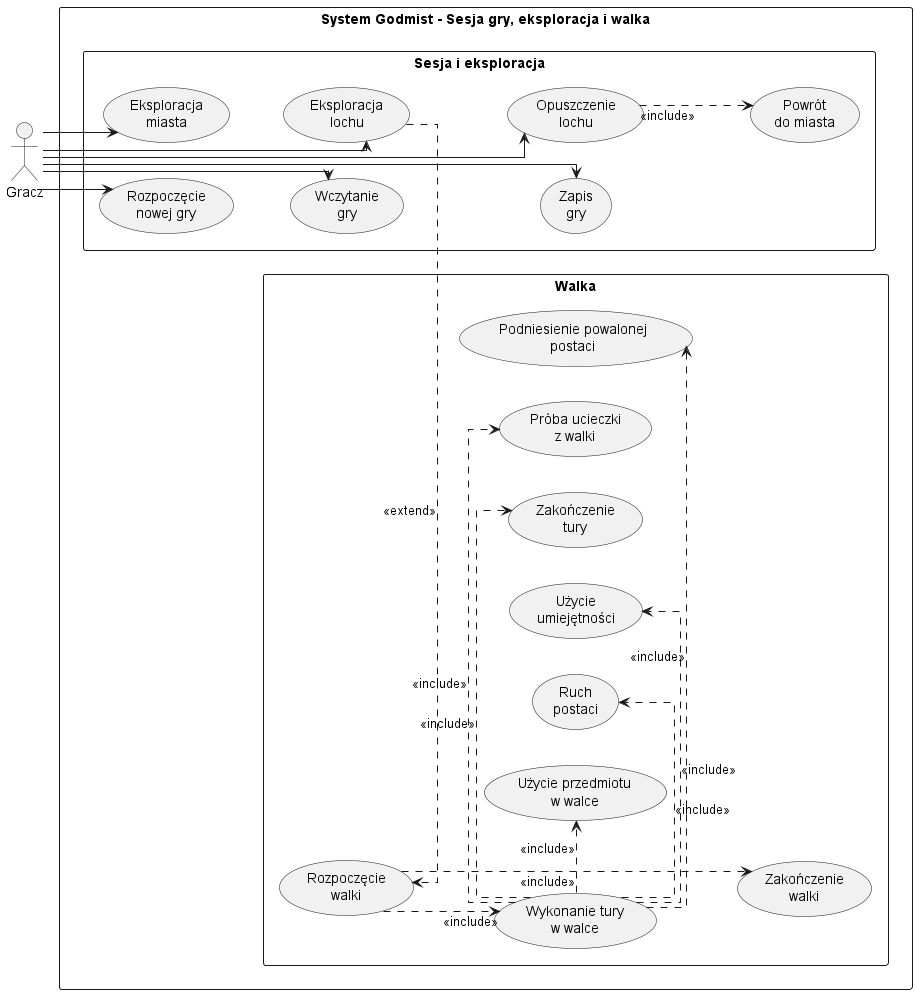
\includegraphics[width=\textwidth,height=0.78\textheight,keepaspectratio]{figures/uml/uc1.png}
    \caption{Diagram przypadków użycia dla sesji gry, eksploracji i walki.}
    \label{fig:use-case-session-exploration-combat}
    \wsizsource{Opracowanie własne}
\end{figure}

Pierwszy diagram przedstawia funkcje związane z rozpoczęciem i obsługą sesji gry, eksploracją miasta i lochu oraz przejściem do systemu walki. Szczególnie istotna jest tu relacja \textit{extend} pomiędzy eksploracją lochu a rozpoczęciem walki, ponieważ pokazuje ona, że walka stanowi zdarzenie uruchamiane w określonym kontekście eksploracji. Diagram obejmuje również podstawowe działania wykonywane w trakcie starcia oraz zakończenie walki i powrót z lochu do miasta.

\begin{figure}[H]
    \centering
    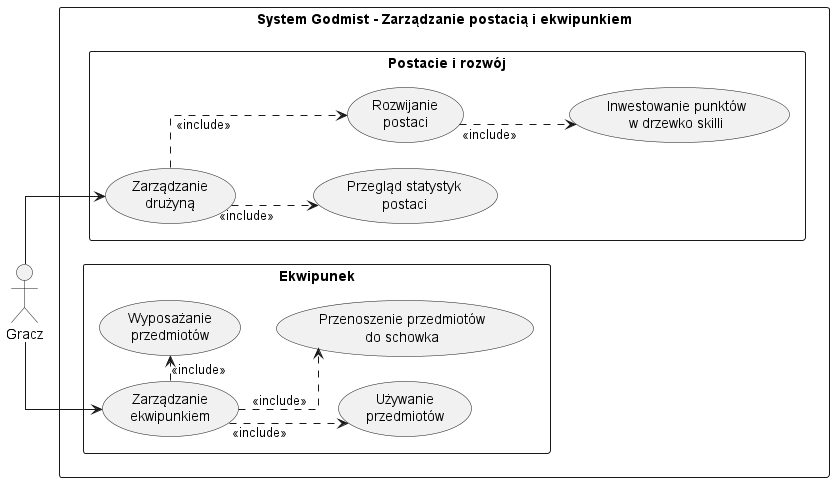
\includegraphics[width=0.9\textwidth,height=0.68\textheight,keepaspectratio]{figures/uml/uc2.png}
    \caption{Diagram przypadków użycia dla zarządzania postacią i ekwipunkiem.}
    \label{fig:use-case-character-inventory}
    \wsizsource{Opracowanie własne}
\end{figure}

Drugi diagram koncentruje się na funkcjach związanych z zarządzaniem drużyną, rozwojem postaci oraz obsługą ekwipunku. Pokazano na nim zależności pomiędzy przeglądem statystyk, rozwijaniem postaci i inwestowaniem punktów w drzewka skilli, a także podstawowe operacje wykonywane na przedmiotach. Diagram ten przedstawia obszar systemu odpowiedzialny za rozwój drużyny oraz organizację zasobów gracza poza bezpośrednim przebiegiem walki.

\begin{figure}[H]
    \centering
    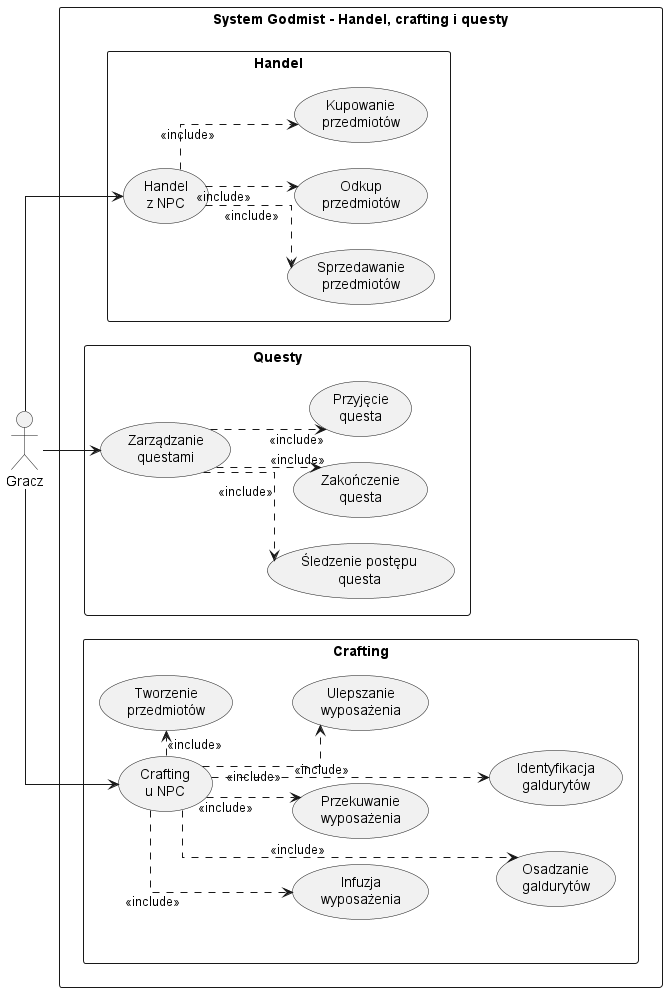
\includegraphics[width=\textwidth,height=0.78\textheight,keepaspectratio]{figures/uml/uc3.png}
    \caption{Diagram przypadków użycia dla handlu, craftingu i questów.}
    \label{fig:use-case-npc-services}
    \wsizsource{Opracowanie własne}
\end{figure}

Trzeci diagram obejmuje funkcje realizowane głównie w interakcji z postaciami niezależnymi, a więc handel, crafting oraz zarządzanie questami. Zostały na nim przedstawione zarówno podstawowe operacje handlowe, jak i bardziej rozbudowane działania związane z ulepszaniem wyposażenia, infuzją oraz obsługą galdurytów. Ujęcie questów w tym samym diagramie wynika z ich silnego powiązania z interakcjami z NPC oraz miejskim zapleczem rozgrywki.
\subsection{Scenariusze przypadków użycia}
\label{subsec:scenariusze-przypadkow-uzycia}

W niniejszym podrozdziale przedstawiono dwa przykładowe scenariusze przypadków użycia dla systemu \emph{Godmist}. Wybrane scenariusze obejmują jeden przypadek związany bezpośrednio z rozgrywką oraz jeden przypadek o charakterze systemowym. Pozwala to pokazać zarówno logikę mechanik gry, jak i obsługę trwałości danych.

\subsubsection*{Scenariusz przypadku użycia: Rozpoczęcie walki}

\textbf{Nazwa przypadku użycia:} Rozpoczęcie walki

\textbf{Aktor główny:} Gracz

\textbf{Cel:} Rozpoczęcie starcia pomiędzy drużyną gracza a przeciwnikami w wyniku eksploracji, interakcji skryptowej lub dialogu.

\textbf{Warunki wstępne:}
\begin{itemize}
    \item gra znajduje się w stanie aktywnej eksploracji miasta lub lochu,
    \item na mapie istnieje grupa jednostek lub zdarzenie mogące wywołać walkę,
    \item stan gry pozwala na przejście do trybu walki.
\end{itemize}

\textbf{Warunki końcowe:}
\begin{itemize}
    \item zostaje utworzona aktywna sesja walki,
    \item uczestnicy walki zostają przypisani do odpowiednich drużyn i relacji,
    \item zostaje wyznaczona kolejność tur,
    \item interfejs użytkownika przechodzi do trybu walki.
\end{itemize}

\textbf{Przebieg główny:}
\begin{enumerate}
    \item Gracz porusza drużyną po mapie lub podejmuje interakcję prowadzącą do starcia.
    \item System wykrywa spełnienie warunku rozpoczęcia walki.
    \item System identyfikuje jednostki biorące udział w starciu.
    \item System wyznacza obszar walki na podstawie miejsca kontaktu i aktualnej mapy.
    \item System tworzy instancję sesji walki.
    \item System przekształca uczestników zdarzenia w jednostki bojowe wraz z ich bieżącym stanem.
    \item System przypisuje uczestników do odpowiednich drużyn oraz określa relacje pomiędzy nimi.
    \item System inicjalizuje parametry walki, w tym pozycje jednostek, aktualne punkty akcji i zasoby.
    \item System wyznacza kolejność tur zgodnie z obowiązującymi regułami.
    \item System przełącza interfejs użytkownika do trybu walki.
    \item System przekazuje sterowanie pierwszej jednostce w kolejności tury.
\end{enumerate}

\textbf{Przebiegi alternatywne:}
\begin{itemize}
    \item Jeżeli walka została wywołana przez dialog, system rozpoczyna starcie po zakończeniu wybranej kwestii dialogowej.
    \item Jeżeli na planszy występują neutralne lub sojusznicze jednostki niezależne, system może dodać je do walki zgodnie z relacjami do drużyn.
    \item Jeżeli starcie przestaje być zasadne jeszcze przed właściwą inicjalizacją, system nie tworzy sesji walki i pozostaje w trybie eksploracji.
\end{itemize}

\textbf{Uwagi:}
\begin{itemize}
    \item rozpoczęcie walki nie przenosi gracza do oddzielnej mapy, lecz wykorzystuje tę samą przestrzeń podzieloną na pola,
    \item pole walki zależy od aktualnego otoczenia, na przykład korytarza, pomieszczenia lub otwartego terenu.
\end{itemize}

\subsubsection*{Scenariusz przypadku użycia: Zapis gry}

\textbf{Nazwa przypadku użycia:} Zapis gry

\textbf{Aktor główny:} Gracz

\textbf{Cel:} Utrwalenie aktualnego stanu gry w pliku zapisu, tak aby można było go później odtworzyć.

\textbf{Warunki wstępne:}
\begin{itemize}
    \item gra znajduje się w stanie, w którym zapis jest dozwolony,
    \item istnieje aktywna kampania lub aktywny stan rozgrywki,
    \item system posiada dostęp do lokalizacji przeznaczonej na pliki zapisu.
\end{itemize}

\textbf{Warunki końcowe:}
\begin{itemize}
    \item aktualny stan gry zostaje zapisany w nowym lub zaktualizowanym wpisie listy zapisów,
    \item metadane zapisu zostają zaktualizowane,
    \item użytkownik otrzymuje informację o powodzeniu lub niepowodzeniu operacji.
\end{itemize}

\textbf{Przebieg główny:}
\begin{enumerate}
    \item Gracz wybiera opcję zapisu gry z poziomu interfejsu systemowego.
    \item System weryfikuje, czy aktualny stan gry pozwala na wykonanie zapisu.
    \item System pobiera bieżący stan postaci, świata, questów, lochów, NPC, schowka i innych istotnych elementów rozgrywki.
    \item System przekształca dane runtime do struktur przeznaczonych do serializacji.
    \item System buduje kompletny obiekt danych zapisu gry.
    \item System serializuje dane do formatu JSON.
    \item System zapisuje dane do pliku.
    \item System aktualizuje metadane zapisu, takie jak data, nazwa lub identyfikator zapisu.
    \item System odświeża listę dostępnych zapisów.
    \item System informuje gracza o poprawnym zakończeniu operacji.
\end{enumerate}

\textbf{Przebiegi alternatywne:}
\begin{itemize}
    \item Jeżeli zapis gry jest niedozwolony w aktualnym stanie, system przerywa operację i wyświetla odpowiedni komunikat.
    \item Jeżeli podczas serializacji lub zapisu pliku wystąpi błąd, system zgłasza niepowodzenie operacji i nie nadpisuje poprawnych wcześniejszych zapisów.
    \item Jeżeli zapis wykonywany jest automatycznie, system pomija część interakcji użytkownika i zapisuje stan zgodnie z regułami autosave.
\end{itemize}

\textbf{Uwagi:}
\begin{itemize}
    \item zapis gry obejmuje zarówno stan postaci i ich wyposażenia, jak i postęp questów, stan świata, lochów oraz informacje o usługach i ofertach NPC,
    \item model zapisu oparty jest na plikach JSON i nie wykorzystuje relacyjnej bazy danych.
\end{itemize}

\subsection{Diagramy aktywności}

\begin{figure}[H]
    \centering
    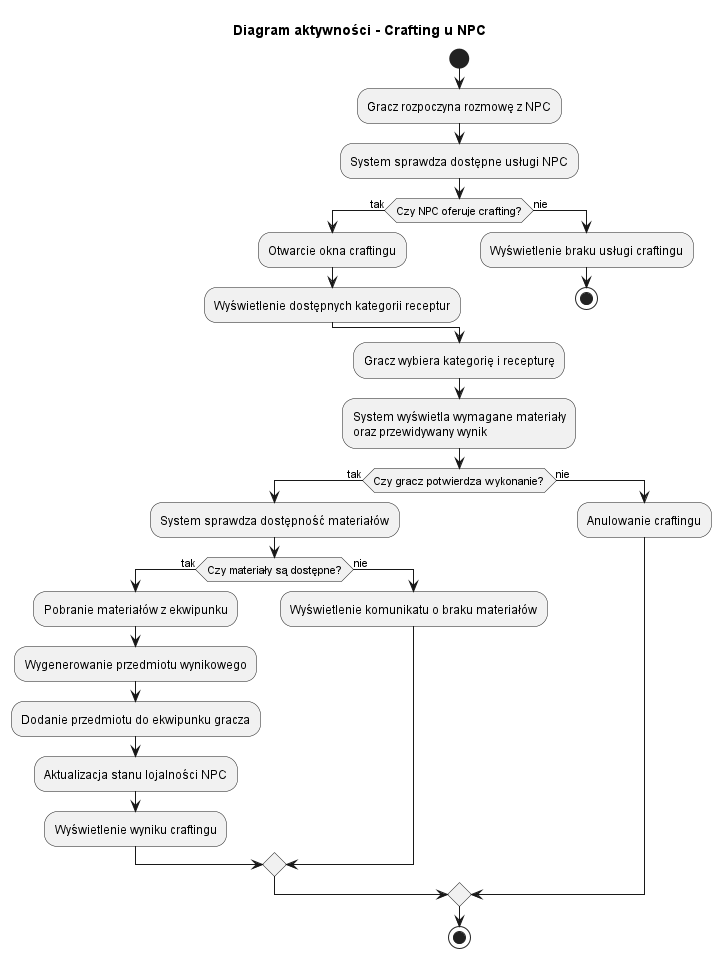
\includegraphics[width=\textwidth,height=0.72\textheight,keepaspectratio]{figures/uml/akt1.png}
    \caption{Diagram aktywności przedstawiający proces craftingu u NPC.}
    \label{fig:activity-crafting-npc}
    \wsizsource{Opracowanie własne}
\end{figure}

Diagram przedstawia przebieg procesu tworzenia przedmiotów z perspektywy gracza i systemu. Uwzględniono w nim zarówno weryfikację dostępności usługi craftingu u danego NPC, jak i sprawdzenie wymaganych materiałów przed wykonaniem operacji. Diagram pokazuje również możliwe ścieżki alternatywne, takie jak brak odpowiedniej usługi lub anulowanie procesu przez gracza.

\begin{figure}[H]
    \centering
    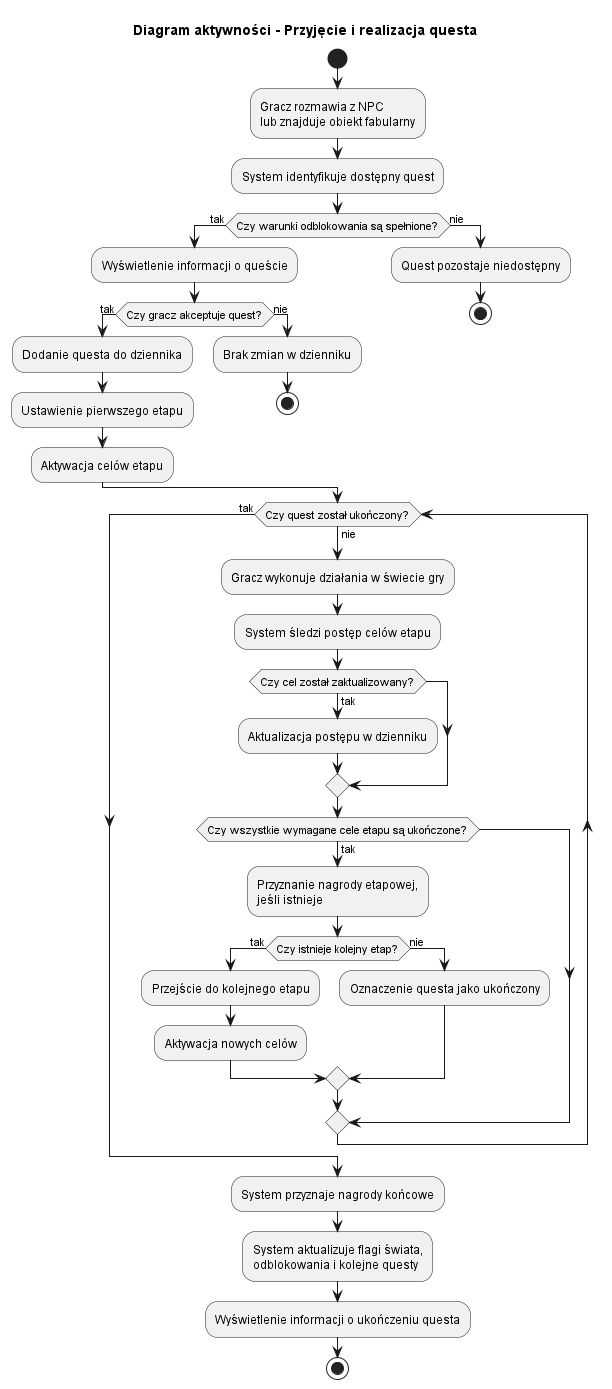
\includegraphics[width=\textwidth,height=0.72\textheight,keepaspectratio]{figures/uml/akt2.png}
    \caption{Diagram aktywności przedstawiający przyjęcie i realizację questa.}
    \label{fig:activity-quest-flow}
    \wsizsource{Opracowanie własne}
\end{figure}

Diagram opisuje pełny cykl życia zadania od momentu jego wykrycia do zakończenia i przyznania nagród. Pokazano na nim mechanizmy sprawdzania warunków odblokowania, akceptacji zadania przez gracza oraz aktualizacji postępu w kolejnych etapach. Ujęto także możliwość przechodzenia do następnych etapów oraz aktualizacji stanu świata po ukończeniu questa.

\subsection{Diagramy sekwencji}

\begin{figure}[H]
    \centering
    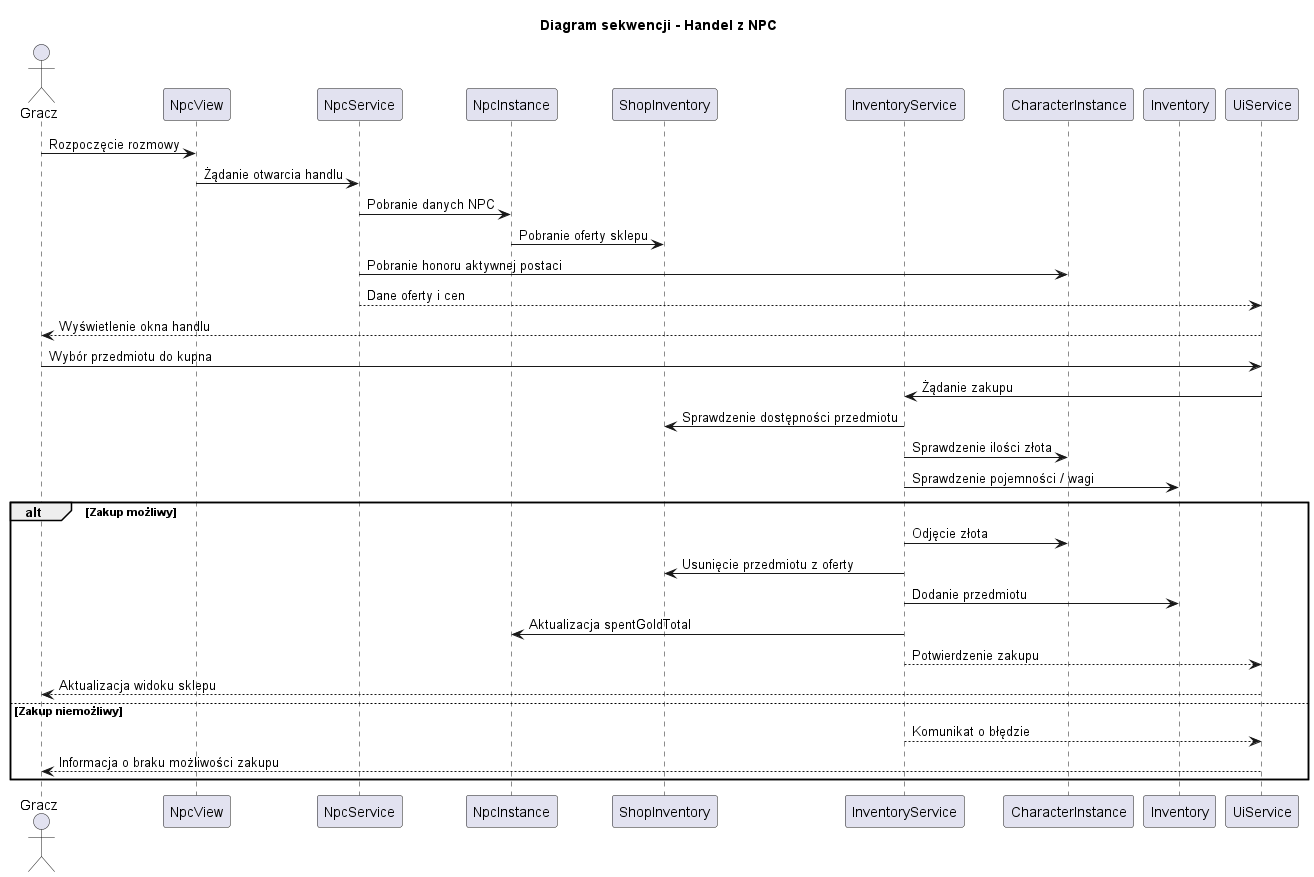
\includegraphics[width=\textwidth,height=0.72\textheight,keepaspectratio]{figures/uml/sek1.png}
    \caption{Diagram sekwencji przedstawiający handel z NPC.}
    \label{fig:sequence-trade-npc}
    \wsizsource{Opracowanie własne}
\end{figure}

Diagram sekwencji pokazuje współpracę pomiędzy interfejsem użytkownika, systemem NPC, ekwipunkiem oraz logiką zakupu podczas handlu. Proces rozpoczyna się od wejścia w interakcję z postacią niezależną i otwarcia okna handlu, a następnie przechodzi do weryfikacji oferty, ilości złota oraz ograniczeń ekwipunku. Diagram uwzględnia zarówno poprawny zakup, jak i sytuację, w której transakcja nie może zostać zrealizowana.

\begin{figure}[H]
    \centering
    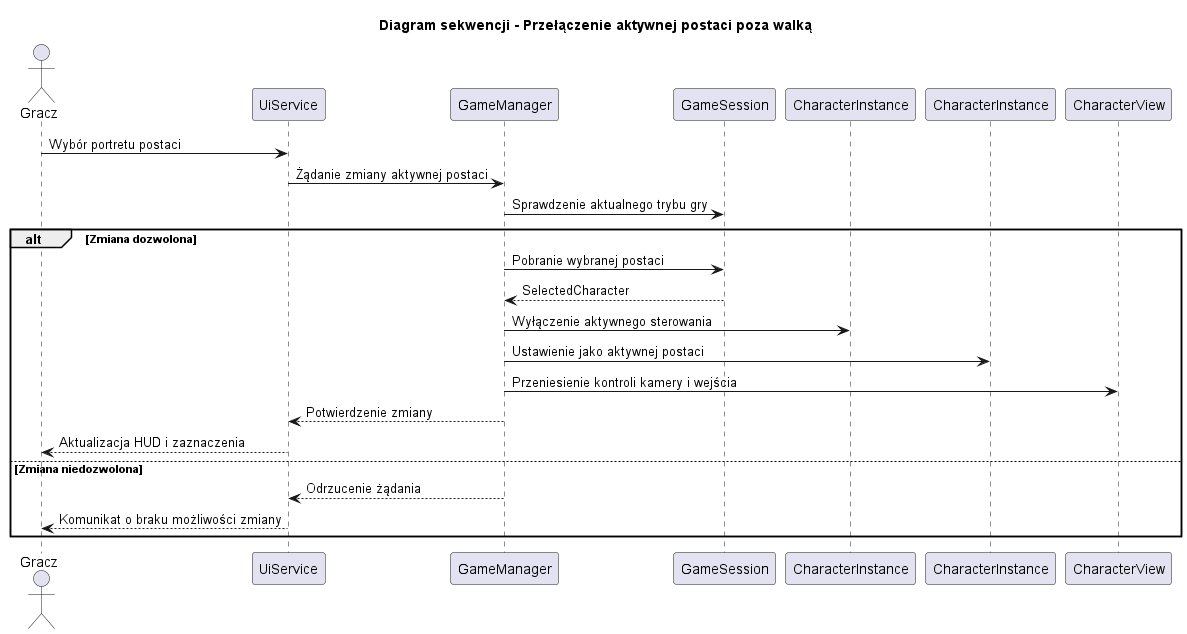
\includegraphics[width=\textwidth,height=0.72\textheight,keepaspectratio]{figures/uml/sek2.png}
    \caption{Diagram sekwencji przedstawiający przełączenie aktywnej postaci poza walką.}
    \label{fig:sequence-switch-active-character}
    \wsizsource{Opracowanie własne}
\end{figure}

Diagram obrazuje proces zmiany aktualnie sterowanej postaci w trybie eksploracji. Pokazano w nim sprawdzenie, czy zmiana jest dozwolona w bieżącym stanie gry, a następnie przekazanie sterowania nowo wybranej postaci oraz aktualizację warstwy prezentacji. Uwzględniono również ścieżkę alternatywną, w której zmiana zostaje odrzucona przez system.

\subsection{Diagramy stanów}

\begin{figure}[H]
    \centering
    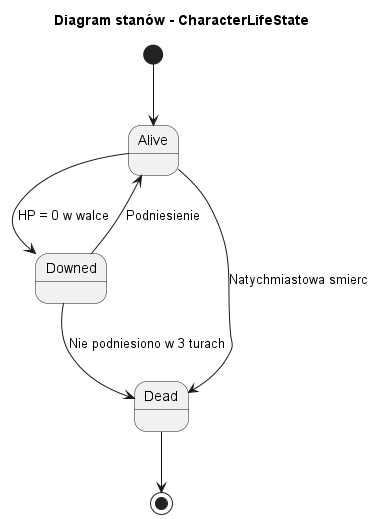
\includegraphics[width=0.75\textwidth,height=0.50\textheight,keepaspectratio]{figures/uml/stan1.png}
    \caption{Diagram stanów obiektu CharacterLifeState.}
    \label{fig:state-character-life}
    \wsizsource{Opracowanie własne}
\end{figure}

Diagram stanów przedstawia możliwe stany życia postaci oraz warunki przejścia pomiędzy nimi. Model obejmuje stan aktywny, powalenie oraz śmierć definitywną, zgodnie z założeniami systemu walki w grze. Szczególnie istotne jest tu przejście ze stanu \textit{Downed} do \textit{Dead}, które następuje, gdy postać nie zostanie podniesiona w ciągu trzech tur.

\begin{figure}[H]
    \centering
    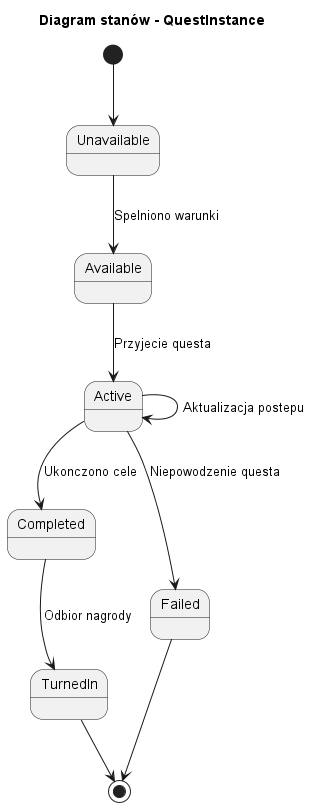
\includegraphics[width=0.82\textwidth,height=0.55\textheight,keepaspectratio]{figures/uml/stan2.png}
    \caption{Diagram stanów obiektu QuestInstance.}
    \label{fig:state-quest-instance}
    \wsizsource{Opracowanie własne}
\end{figure}

Diagram opisuje zmiany stanu instancji zadania w trakcie jego udostępniania, realizacji i zamykania. Uwzględniono w nim etap odblokowania zadania, jego przyjęcie, aktualizację postępu, ukończenie oraz odbiór nagrody. Model przewiduje również możliwość niepowodzenia zadania, co pozwala odwzorować bardziej złożone przebiegi misji w systemie questów.
\section{Technologie i wymagania sprzętowe}
\label{sec:technologie-i-wymagania}

Wybór technologii zastosowanych w projekcie \emph{Godmist} wynika z charakteru systemu oraz założonego zakresu funkcjonalnego. Projektowana aplikacja jest grą komputerową typu single player, łączącą eksplorację lochów, walkę turową, rozwój postaci, system przedmiotów, crafting, interakcje z NPC oraz trwały zapis postępu użytkownika. Oznacza to konieczność zastosowania narzędzi, które umożliwiają zarówno budowę warstwy wizualnej i interaktywnej, jak i czytelne modelowanie logiki systemu oraz trwałości danych.

W niniejszej sekcji przedstawiono główne technologie planowane do wykorzystania w projekcie oraz orientacyjne wymagania sprzętowe dla uruchomienia systemu. Ze względu na fakt, że projekt znajduje się na etapie dokumentacji i modelowania, część parametrów technicznych ma charakter założeń wstępnych i może zostać doprecyzowana na dalszych etapach implementacji.

\subsection{Technologie}
\label{subsec:technologie}

Podstawową technologią zastosowaną w projekcie jest silnik \emph{Unity}. Został on wybrany ze względu na szerokie możliwości tworzenia gier 2D, dobrą integrację warstwy wizualnej z logiką systemu oraz wygodny model pracy oparty na scenach, komponentach i obiektach. Unity umożliwia również stosowanie wzorców architektonicznych wspierających rozdzielenie definicji danych, logiki runtime oraz warstwy prezentacji, co jest istotne z punktu widzenia utrzymania porządku w projekcie.

Językiem implementacji systemu jest \emph{C\#}. Wybór ten wynika bezpośrednio z integracji z silnikiem Unity, ale również z cech samego języka, takich jak obiektowy model programowania, dobra organizacja kodu, możliwość modelowania złożonych struktur danych oraz wygodne tworzenie klas domenowych, serwisów i warstw pośrednich. W projekcie zakłada się szerokie wykorzystanie klas reprezentujących zarówno definicje danych, jak i zmienny stan rozgrywki.

Ważnym elementem architektury systemu jest wykorzystanie obiektów \texttt{ScriptableObject}. Mechanizm ten pozwala przechowywać definicje statycznych danych gry, takich jak klasy postaci, definicje przedmiotów, umiejętności, questy czy definicje lochów. Dzięki temu możliwe jest oddzielenie danych konfiguracyjnych od runtime'owego stanu gry oraz łatwiejsze rozwijanie projektu bez konieczności wprowadzania wszystkich zmian bezpośrednio w kodzie źródłowym.

Do przechowywania stanu gry planowane jest zastosowanie plików \emph{JSON}. Rozwiązanie to jest odpowiednie dla gry single player, w której nie ma potrzeby wykorzystywania zewnętrznej, relacyjnej bazy danych. Zapis w formacie JSON umożliwia przechowywanie stanu postaci, misji, NPC, lochów, ekwipunku i innych elementów w sposób strukturalny i łatwy do odtworzenia. Model ten dobrze współgra z projektowaną architekturą opartą na identyfikatorach definicji i klasach runtime.

W procesie projektowania wykorzystywane są również diagramy UML oraz narzędzia do modelowania wizualnego. Ich zadaniem jest uporządkowanie struktury systemu i przedstawienie zależności pomiędzy jego elementami jeszcze przed pełną implementacją. Dzięki temu możliwe jest wczesne wykrywanie niespójności oraz bardziej świadome planowanie podziału systemu na moduły.

Można zatem przyjąć, że główny stos technologiczny projektu obejmuje:
\begin{itemize}
    \item silnik \emph{Unity},
    \item język programowania \emph{C\#},
    \item definicje danych oparte na \texttt{ScriptableObject},
    \item zapis stanu gry w plikach \emph{JSON},
    \item modelowanie projektowe z użyciem diagramów UML.
\end{itemize}

\subsection{Wymagania sprzętowe}
\label{subsec:wymagania-sprzetowe}

Projektowany system przeznaczony jest do uruchamiania na komputerach osobistych. Ze względu na charakter gry 2D oraz brak rozbudowanych wymagań związanych z renderingiem trójwymiarowym, nie przewiduje się bardzo wysokich wymagań sprzętowych. Jednocześnie system powinien działać stabilnie przy obsłudze walk wieloobiektowych, stanu drużyny, ekwipunku, lochów proceduralnych oraz mechanizmu zapisu i odczytu danych.

Na obecnym etapie projektu można przyjąć orientacyjne wymagania minimalne:
\begin{itemize}
    \item system operacyjny: Windows 10 lub nowszy,
    \item procesor: 64-bitowy, dwurdzeniowy,
    \item pamięć RAM: 8 GB,
    \item karta graficzna: zgodna z DirectX 11,
    \item wolne miejsce na dysku: co najmniej 2 GB.
\end{itemize}

Orientacyjne wymagania zalecane można określić następująco:
\begin{itemize}
    \item system operacyjny: Windows 10 lub nowszy,
    \item procesor: 64-bitowy, czterordzeniowy,
    \item pamięć RAM: 16 GB,
    \item karta graficzna: dedykowana karta obsługująca DirectX 11 lub nowszy,
    \item wolne miejsce na dysku: 4 GB lub więcej.
\end{itemize}

Wymagania te mają charakter wstępny i mogą ulec zmianie w zależności od ostatecznego zakresu implementacji, liczby zasobów graficznych, rozbudowy GUI oraz stopnia złożoności finalnych mechanik. Na obecnym etapie stanowią one jednak wystarczającą podstawę do określenia docelowej platformy działania systemu.

\section{Struktura systemu}
\label{sec:struktura-systemu}

Struktura systemu \emph{Godmist} została zaprojektowana w sposób warstwowy i modularny. Jest to szczególnie istotne ze względu na złożoność projektowanej gry, która łączy wiele współdziałających podsystemów, takich jak eksploracja lochów, walka turowa, rozwój postaci, ekwipunek, crafting, interakcje z NPC, system misji oraz trwałość stanu gry. Przyjęta organizacja rozwiązania ma umożliwiać nie tylko poprawne działanie systemu, ale również jego późniejszą rozbudowę i utrzymanie.

Projekt nie opiera się na klasycznej architekturze bazodanowej charakterystycznej dla systemów biznesowych lub aplikacji sieciowych. Zamiast tego wykorzystuje strukturę danych dopasowaną do gry single player, w której istotną rolę odgrywają definicje statyczne, zmienny stan runtime oraz zapis trwały odtwarzany pomiędzy sesjami użytkownika. Oznacza to konieczność rozdzielenia tych trzech poziomów odpowiedzialności i opisania ich w sposób uporządkowany.

\subsection{Opis modelu danych i trwałości}
\label{subsec:opis-modelu-danych}

W projekcie \emph{Godmist} przyjęto model danych oparty na rozdzieleniu definicji systemowych od danych runtime oraz trwałego zapisu stanu gry. Takie podejście pozwala uniknąć mieszania danych statycznych, które definiują reguły świata gry, z danymi zmiennymi, które opisują bieżący stan rozgrywki konkretnego użytkownika.

Pierwszą warstwę stanowią definicje statyczne. Są to dane opisujące elementy gry, które nie zmieniają się dynamicznie w ramach jednej kampanii, lecz pełnią rolę wzorców wykorzystywanych przez system. Do tej grupy należą między innymi definicje postaci, klas postaci, umiejętności, przedmiotów, NPC, questów i lochów. W architekturze projektu dane tego typu są reprezentowane jako obiekty \texttt{ScriptableObject}, co pozwala na ich czytelną organizację i łatwe rozwijanie w środowisku Unity.

Drugą warstwę stanowią dane runtime, czyli bieżący stan gry podczas działania aplikacji. Warstwa ta obejmuje między innymi stan postaci, aktywne questy, stan lochu, ekwipunek, relacje między drużynami w walce, efekty pasywne oraz aktualne położenie i stan obiektów świata. Dane te są modyfikowane w trakcie rozgrywki i odzwierciedlają aktualną sytuację użytkownika.

Trzecią warstwę stanowi trwałość danych, czyli sposób zapisu i odtwarzania stanu gry pomiędzy sesjami. W projekcie nie zastosowano klasycznej relacyjnej bazy danych. Zamiast tego zapis realizowany jest z wykorzystaniem plików \emph{JSON}. Rozwiązanie to jest uzasadnione charakterem gry single player, brakiem konieczności komunikacji z centralnym serwerem oraz potrzebą wygodnego odtwarzania rozbudowanego stanu gry. W zapisie przechowywane są między innymi dane postaci, stany przedmiotów, questów, NPC, lochów, schowka i świata.

Istotnym założeniem modelu danych jest identyfikowanie obiektów logicznych za pomocą stabilnych identyfikatorów tekstowych. Dzięki temu możliwe jest odwoływanie się do definicji danych oraz rekonstrukcja zależności pomiędzy obiektami podczas wczytywania gry. Przykładowo postać może odnosić się do definicji swojej klasy, przedmiot do definicji typu przedmiotu, a quest do definicji etapu lub celu. Takie podejście upraszcza serializację danych i wspiera modularny charakter projektu.

W przypadku lochów proceduralnych zastosowano podejście oparte na przechowywaniu ziarna generowania oraz zmian względem stanu bazowego. Oznacza to, że zamiast zapisywania pełnej, surowej kopii każdego elementu runtime, system może odtwarzać strukturę lochu na podstawie parametrów generacji i zapamiętanych różnic, takich jak odwiedzone pomieszczenia, pokonane walki czy aktywowane obiekty. Pozwala to ograniczyć złożoność zapisu i lepiej dopasować model trwałości do charakteru gry.

\subsection{Diagram ERD}
\label{subsec:diagram-erd}

\begin{figure}[H]
    \centering
    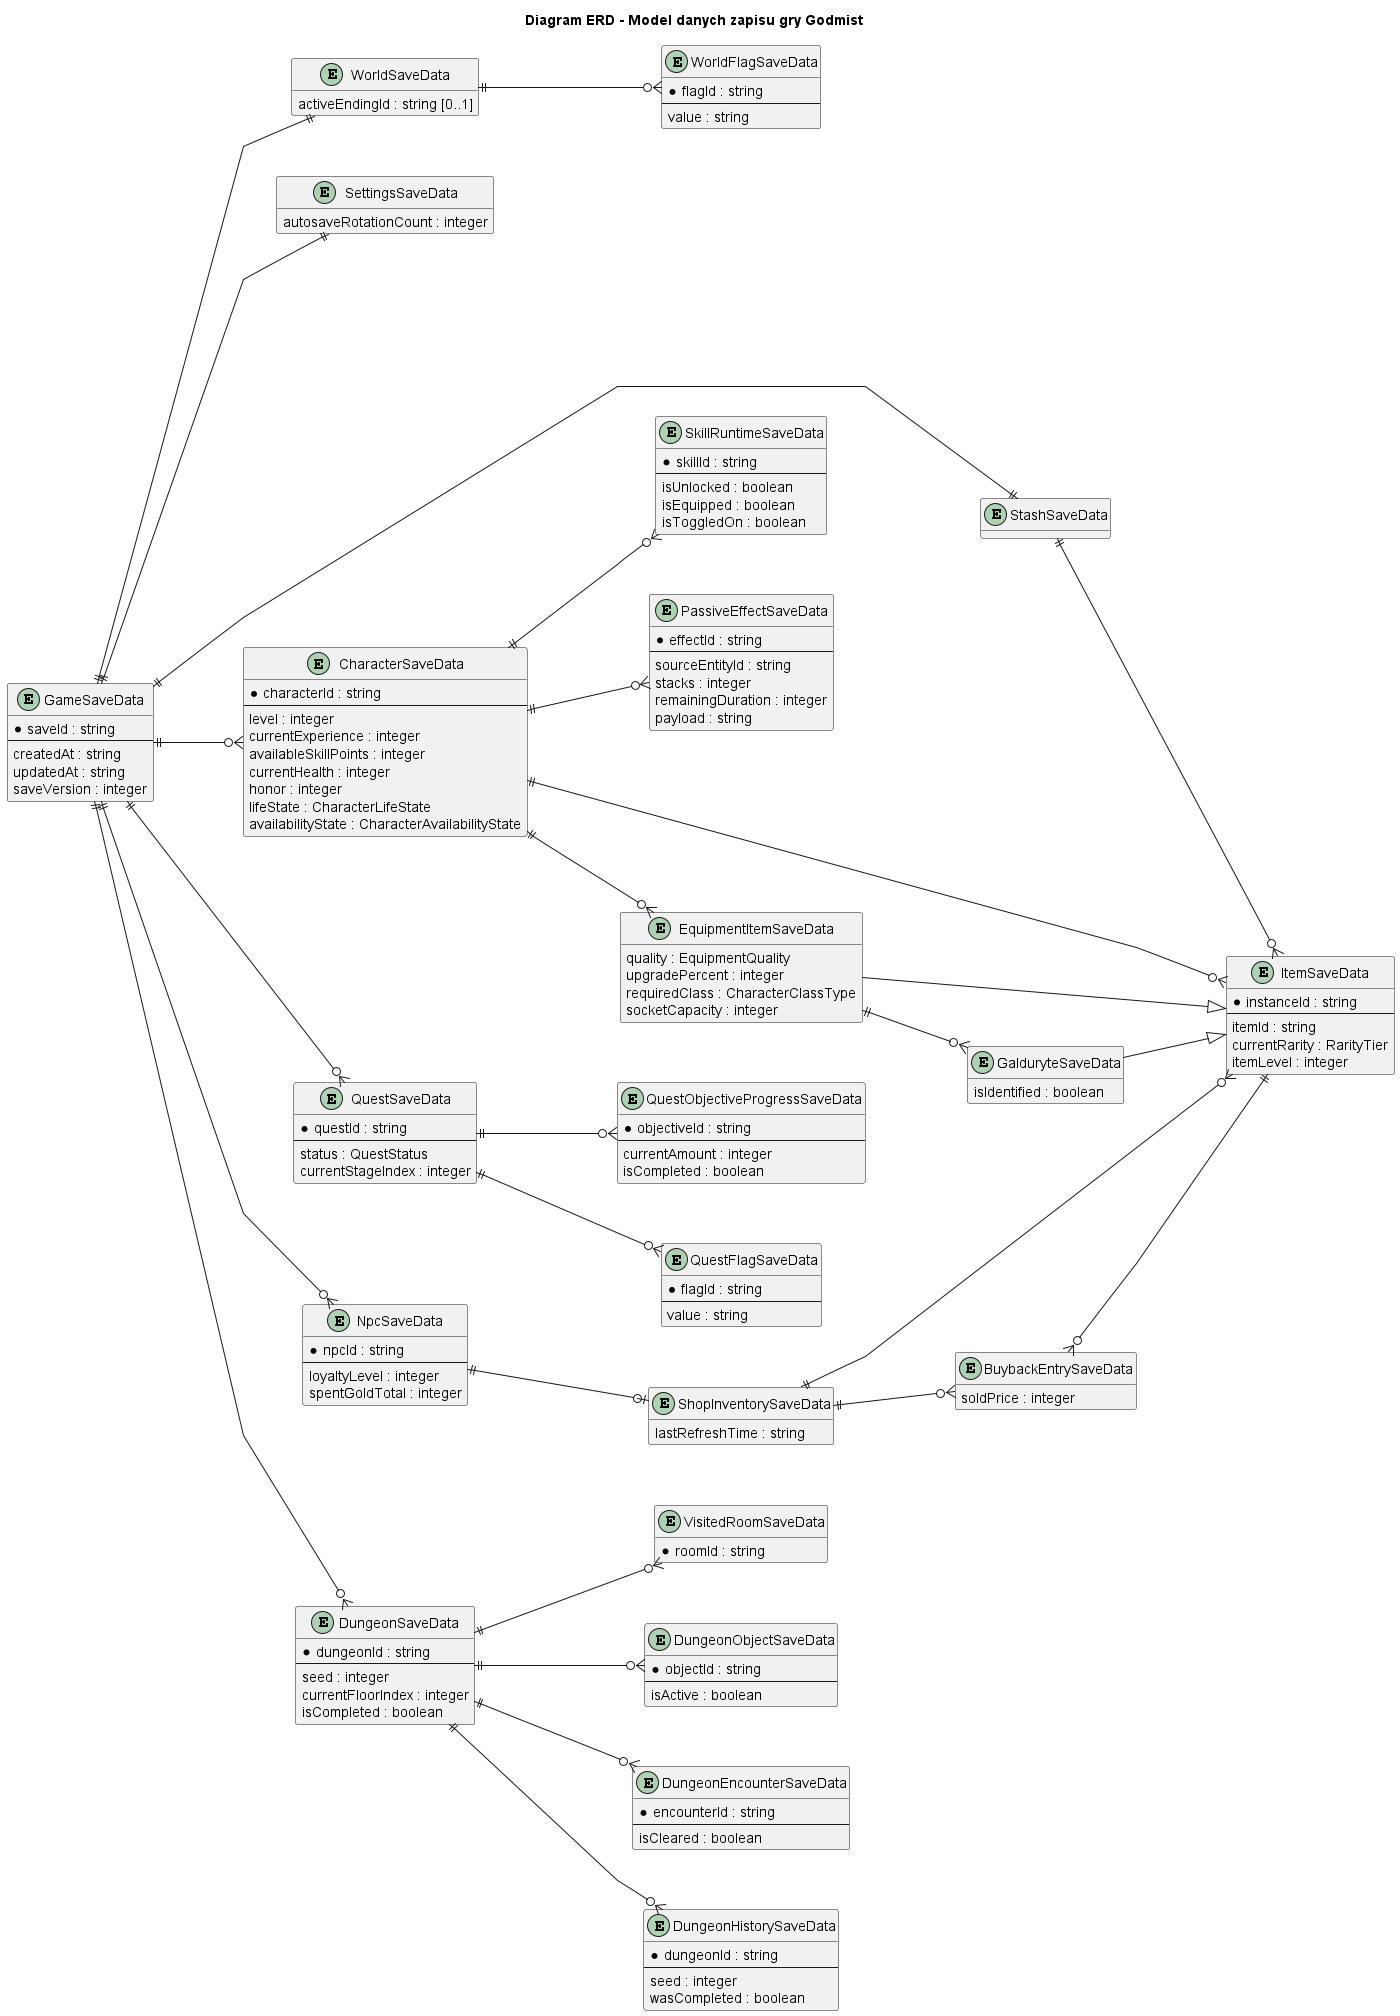
\includegraphics[width=\textwidth,height=0.82\textheight,keepaspectratio]{figures/uml/erd.png}
    \caption{Diagram ERD logicznego modelu danych zapisu gry Godmist.}
    \label{fig:erd-godmist}
    \wsizsource{Opracowanie własne}
\end{figure}

Ze względu na charakter projektowanego systemu diagram ERD nie przedstawia klasycznej relacyjnej bazy danych, lecz logiczny model encji i zależności wykorzystywanych do zapisu stanu gry. Ujęto na nim najważniejsze struktury trwałe, takie jak zapis globalny, stan świata, postacie, questy, NPC, lochy oraz dane związane z przedmiotami i schowkiem. Diagram pokazuje również relacje właścicielskie pomiędzy głównym obiektem zapisu a jego elementami składowymi, a także zależności pomiędzy specjalizacjami danych przedmiotów. Taka forma modelu danych lepiej odpowiada architekturze gry single player wykorzystującej pliki JSON niż klasyczny schemat tabel relacyjnych.

\subsection{Diagram klas}
\label{subsec:diagram-klas}

\begin{figure}[H]
    \centering
    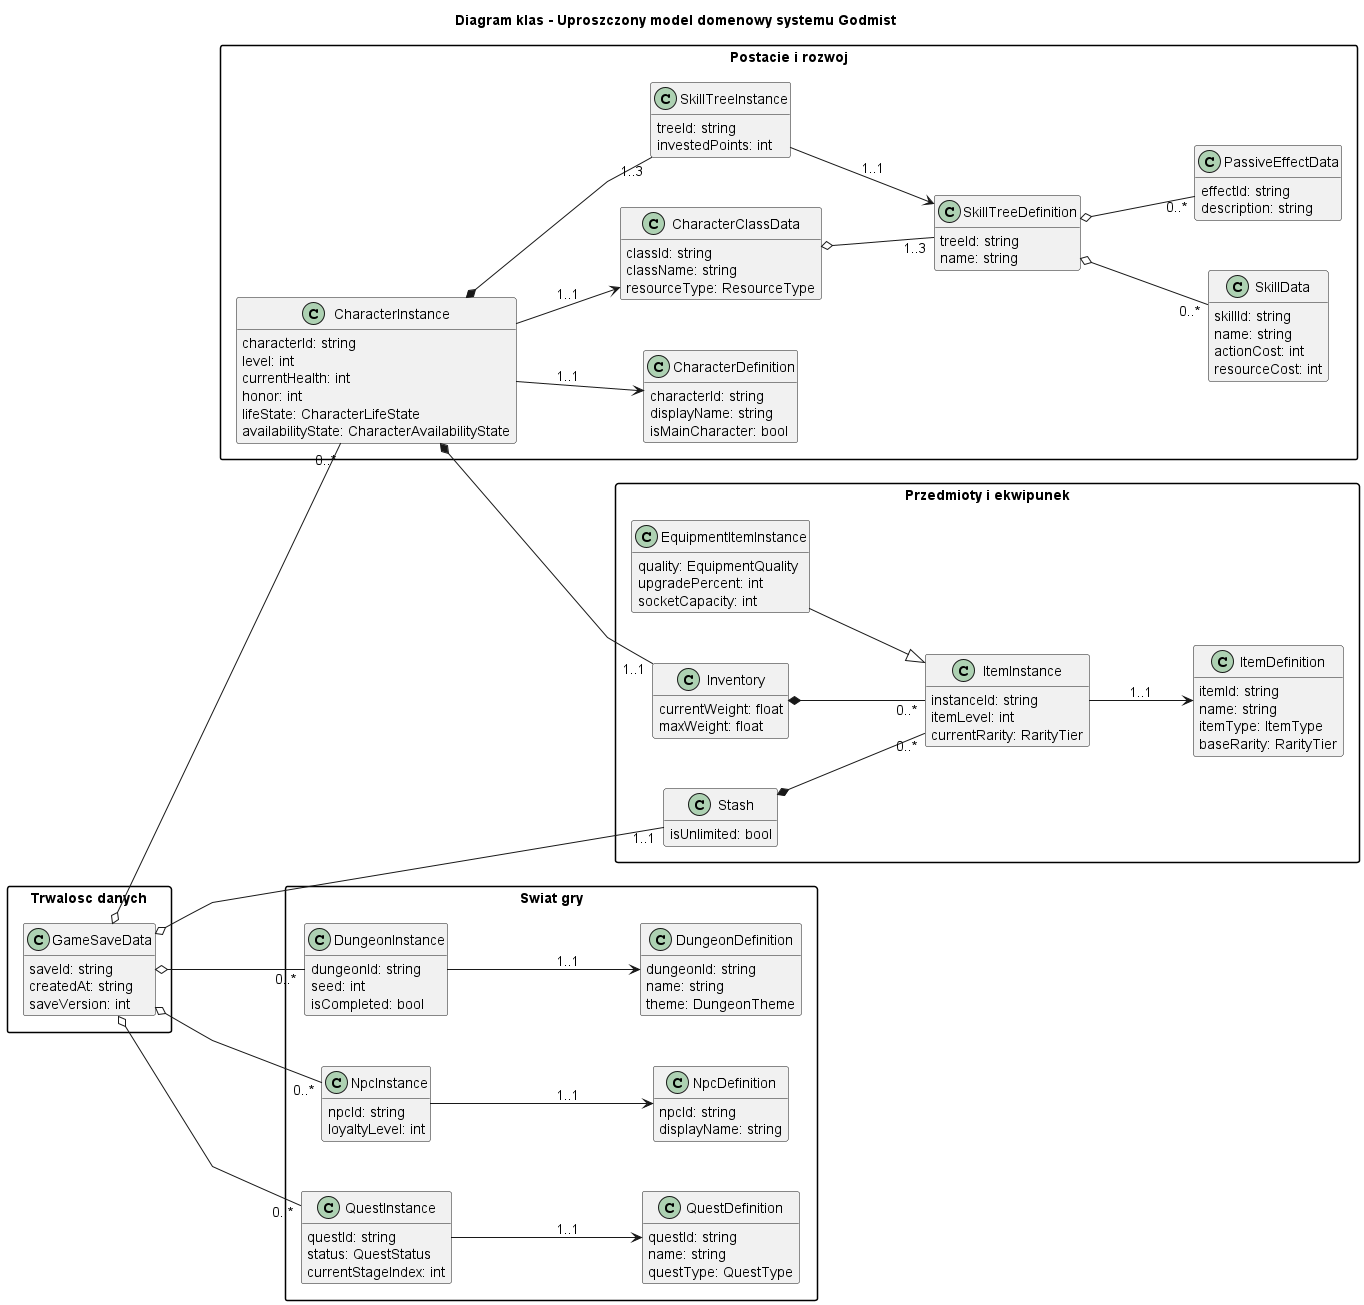
\includegraphics[width=\textwidth,height=0.82\textheight,keepaspectratio]{figures/uml/class-diagram.png}
    \caption{Uproszczony diagram klas systemu Godmist.}
    \label{fig:class-diagram-godmist}
    \wsizsource{Opracowanie własne}
\end{figure}

Na potrzeby niniejszej dokumentacji przedstawiono uproszczony diagram klas, którego celem jest pokazanie najważniejszych klas domenowych systemu oraz zależności pomiędzy nimi. Diagram nie stanowi pełnego odwzorowania wszystkich klas projektowych i implementacyjnych, lecz syntetyczny model obejmujący kluczowe obszary systemu: postacie i rozwój, przedmioty i ekwipunek, świat gry oraz trwałość danych. Takie uproszczenie zostało zastosowane celowo, aby zachować czytelność modelu i umożliwić jego analizę na poziomie architektury logicznej systemu.

Na diagramie widoczne są zależności pomiędzy definicjami danych, instancjami runtime oraz głównym obiektem zapisu gry. Pokazano między innymi relacje pomiędzy definicją postaci a jej instancją, powiązania klas postaci z drzewkami rozwoju, zależności pomiędzy instancjami przedmiotów i ich definicjami, a także relacje łączące zapis gry ze stanem postaci, questów, NPC, lochu i schowka. Dzięki temu diagram stanowi podsumowanie struktury domenowej systemu i uzupełnia wcześniejsze modele zachowania oraz model danych trwałych przedstawiony na diagramie ERD.

Warto podkreślić, że na diagramie pominięto część klas pomocniczych i szczegółowych mechanizmów, takich jak klasy widoku, serwisy systemowe, szczegółowe klasy walki, niższopoziomowe struktury zapisu oraz wybrane obiekty pomocnicze związane z mechanikami specjalistycznymi. Zabieg ten pozwolił skupić się na relacjach najistotniejszych z perspektywy projektowej i inżynierskiej. W efekcie diagram klas pełni w pracy rolę modelu poglądowego, porządkującego logikę architektury systemu, a nie pełnej dokumentacji implementacyjnej wszystkich elementów projektu.

\subsection{Architektura warstwowa systemu}
\label{subsec:architektura-warstwowa}

Projekt \emph{Godmist} wykorzystuje architekturę warstwową, której celem jest rozdzielenie odpowiedzialności pomiędzy definicje danych, logikę domenową, serwisy systemowe oraz warstwę prezentacji. Takie podejście jest szczególnie korzystne w środowisku Unity, ponieważ pozwala ograniczyć nadmierne mieszanie logiki gry z klasami odpowiedzialnymi za scenę, widok i wejście użytkownika.

Pierwszą warstwę stanowią definicje danych. Obejmuje ona obiekty \texttt{ScriptableObject}, które przechowują statyczne informacje o klasach postaci, umiejętnościach, questach, przedmiotach, NPC i lochach. Warstwa ta pełni funkcję konfiguracji systemu i nie reprezentuje bezpośrednio zmiennego stanu rozgrywki.

Drugą warstwę stanowi model domenowy runtime. W jej skład wchodzą klasy reprezentujące aktualny stan postaci, walki, lochu, NPC, questów oraz innych elementów rozgrywki. To właśnie ta warstwa odpowiada za odwzorowanie bieżącej sytuacji w grze i przechowuje dane, które ulegają zmianom w trakcie działania aplikacji.

Trzecią warstwę tworzą serwisy systemowe. Ich zadaniem jest koordynowanie działania poszczególnych obszarów funkcjonalnych, takich jak walka, eksploracja, questy, inventory, crafting, NPC czy zapis gry. Serwisy te nie pełnią roli widoków ani definicji danych, lecz realizują logikę operacyjną i pośredniczą pomiędzy stanem gry a interakcjami użytkownika.

Czwartą warstwę stanowi warstwa prezentacji. Obejmuje ona klasy \texttt{MonoBehaviour}, które odpowiadają za wyświetlanie obiektów na scenie, obsługę interakcji użytkownika, integrację z UI oraz reagowanie na zmiany stanu systemu. W tej warstwie mieszczą się między innymi widoki postaci, NPC, obiektów lochu i okien interfejsu użytkownika.

Uzupełnieniem całej architektury jest warstwa trwałości danych, odpowiedzialna za serializację i deserializację stanu gry. Obejmuje ona klasy DTO wykorzystywane do zapisu w formacie JSON oraz komponenty odpowiedzialne za koordynację operacji zapisu i odczytu. Dzięki temu model definicji, runtime i trwałości pozostaje rozdzielony, co poprawia czytelność rozwiązania i ogranicza ryzyko niekontrolowanego przenikania się odpowiedzialności pomiędzy modułami.

Przyjęty podział warstwowy wspiera dalszy rozwój projektu, ponieważ umożliwia niezależną rozbudowę poszczególnych obszarów systemu. Pozwala również łatwiej identyfikować zależności pomiędzy elementami rozwiązania oraz zachować większą kontrolę nad architekturą w miarę wzrostu złożoności gry.

\section{Podsumowanie rozdziału}
\label{sec:podsumowanie-rozdzialu-2}

W niniejszym rozdziale przedstawiono projekt systemu \emph{Godmist} z perspektywy modelowania, doboru technologii oraz organizacji struktury rozwiązania. Omówiono rolę modeli UML jako narzędzia służącego do opisu zachowania i struktury systemu, wskazano główne technologie planowane do wykorzystania w projekcie oraz scharakteryzowano sposób organizacji danych i trwałości stanu gry.

Szczególną uwagę zwrócono na fakt, że projekt nie wykorzystuje klasycznej relacyjnej bazy danych, lecz opiera się na rozdzieleniu definicji statycznych, stanu runtime oraz zapisu trwałego realizowanego z użyciem plików JSON. Pozwoliło to przedstawić architekturę rozwiązania w sposób lepiej dopasowany do charakteru gry single player oraz do przyjętych założeń technologicznych.

Przedstawiona struktura systemu stanowi podstawę do dalszego opisu bardziej praktycznych aspektów projektu. W kolejnym rozdziale omówiony zostanie interfejs użytkownika, propozycje testów oraz końcowe wnioski dotyczące projektowanego rozwiązania.

\chapter{Interfejs użytkownika, testy i podsumowanie}
\label{cha:gui-testy-podsumowanie}

\section{Projekt interfejsu użytkownika}

Interfejs użytkownika gry Godmist zaprojektowano zgodnie z zasadą minimalnej ingerencji w scenę gry. W widokach eksploracji oraz walki większość ekranu zajmuje właściwa scena, natomiast elementy HUD rozmieszczono przy krawędziach ekranu w formie lekkich widżetów. Bardziej rozbudowane okna, takie jak ekwipunek, dziennik zadań czy interakcje z NPC, otwierane są jako osobne nakładki.

\begin{figure}[H]
    \centering
    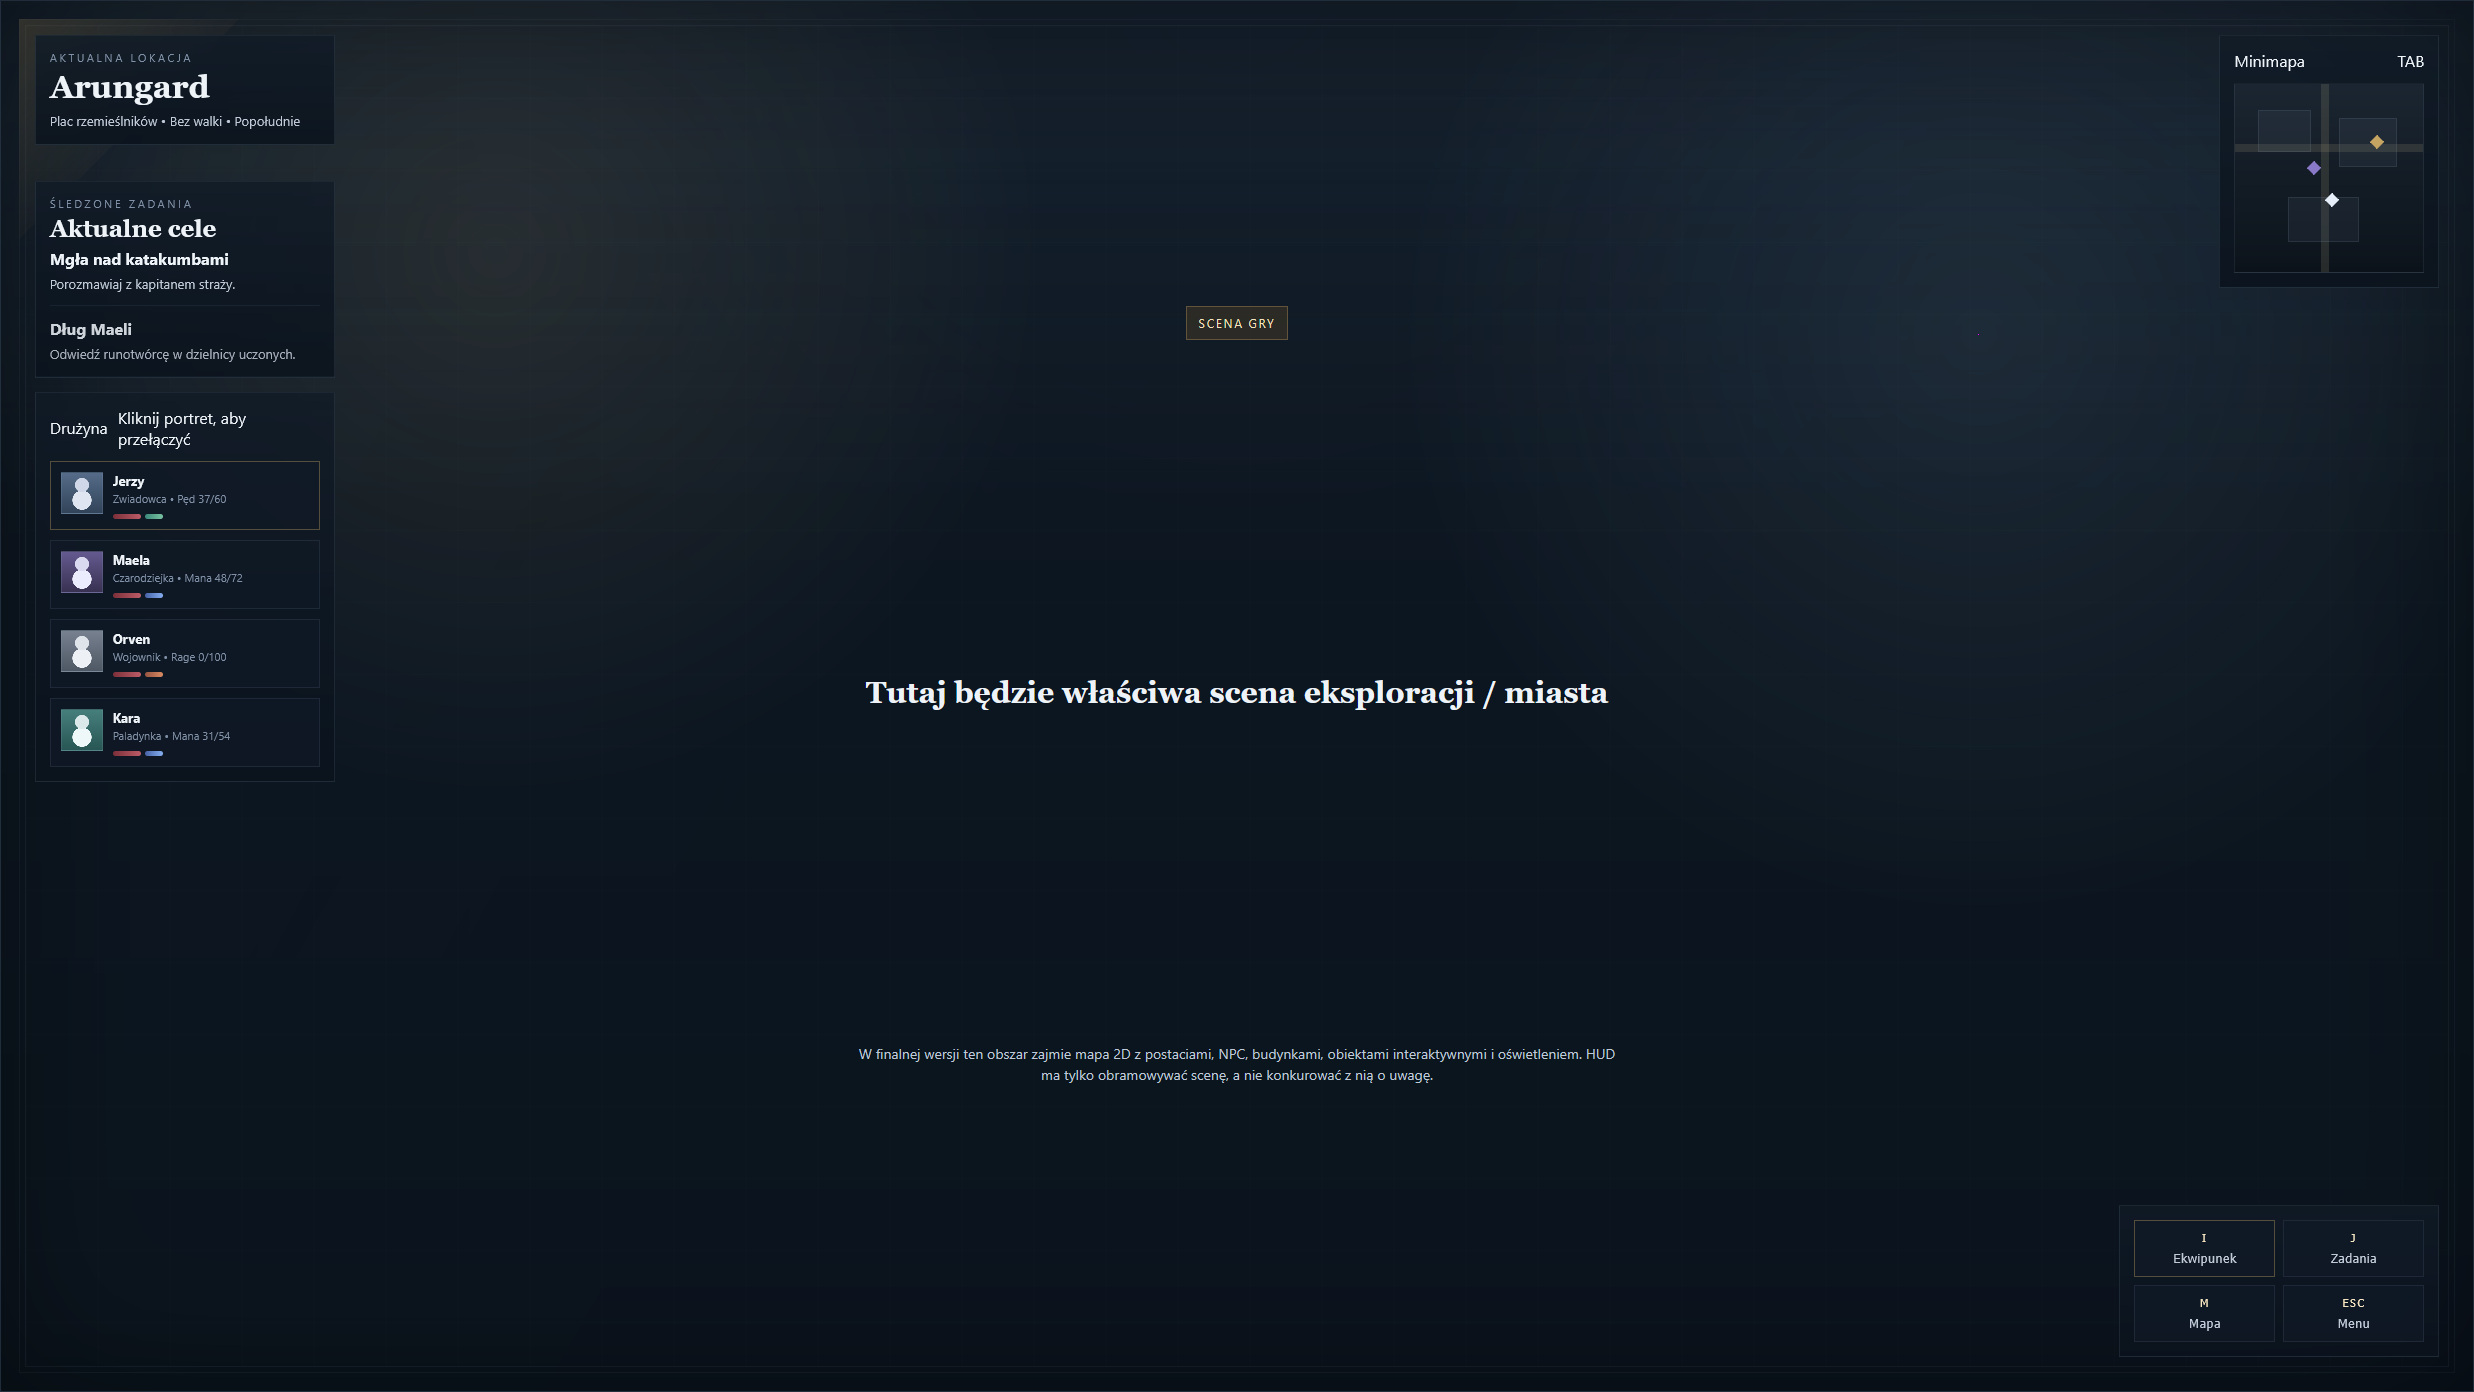
\includegraphics[width=\textwidth]{figures/gui/ui-exploration.png}
    \caption{Widok eksploracji i miasta}
    \wsizsource{Opracowanie własne}
\end{figure}

Widok eksploracji przedstawia podejście scene-first, w którym interfejs ograniczono do najważniejszych informacji: minimapy, aktywnych zadań, składu drużyny oraz podstawowych skrótów. Dzięki temu ekran nie zasłania przestrzeni gry i pozwala skupić uwagę użytkownika na otoczeniu.

\begin{figure}[H]
    \centering
    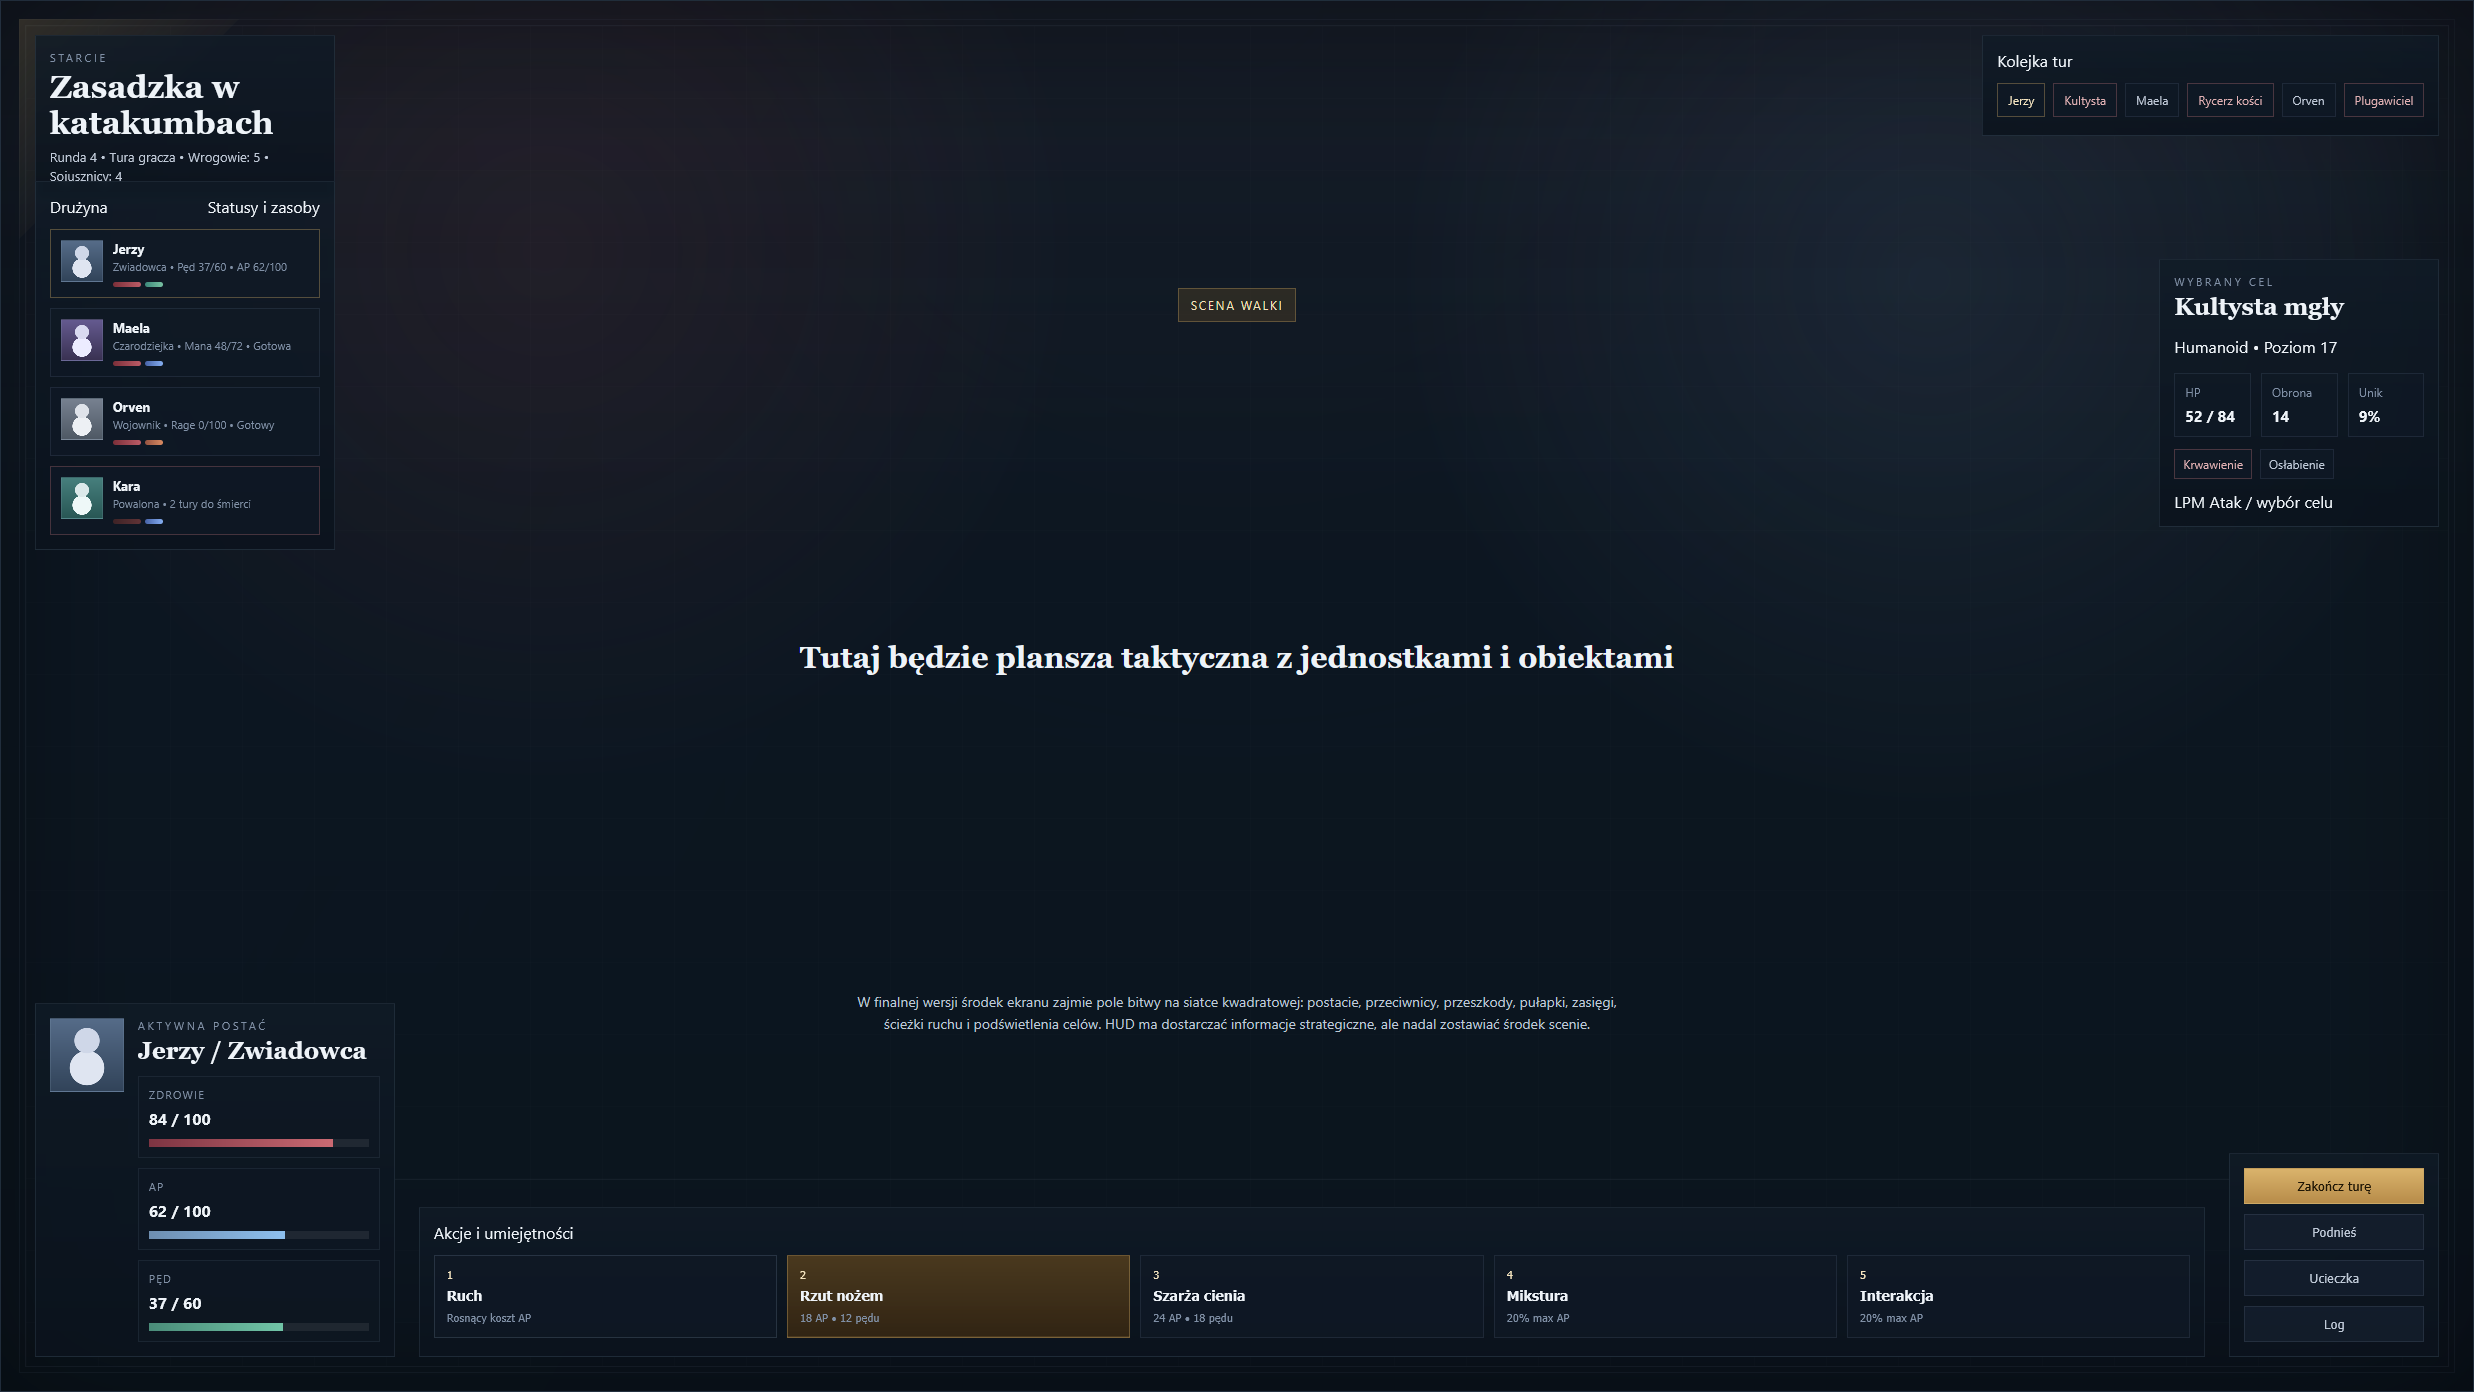
\includegraphics[width=\textwidth]{figures/gui/ui-combat-hud.png}
    \caption{Widok interfejsu walki}
    \wsizsource{Opracowanie własne}
\end{figure}

Interfejs walki zachowuje tę samą zasadę, jednak wzbogacono go o elementy strategiczne, takie jak kolejka tur, pasek umiejętności, panel aktywnej postaci oraz informacje o aktualnym celu. Rozmieszczenie tych elementów przy obrzeżach ekranu umożliwia jednoczesne śledzenie sytuacji taktycznej oraz samego pola bitwy.

\begin{figure}[H]
    \centering
    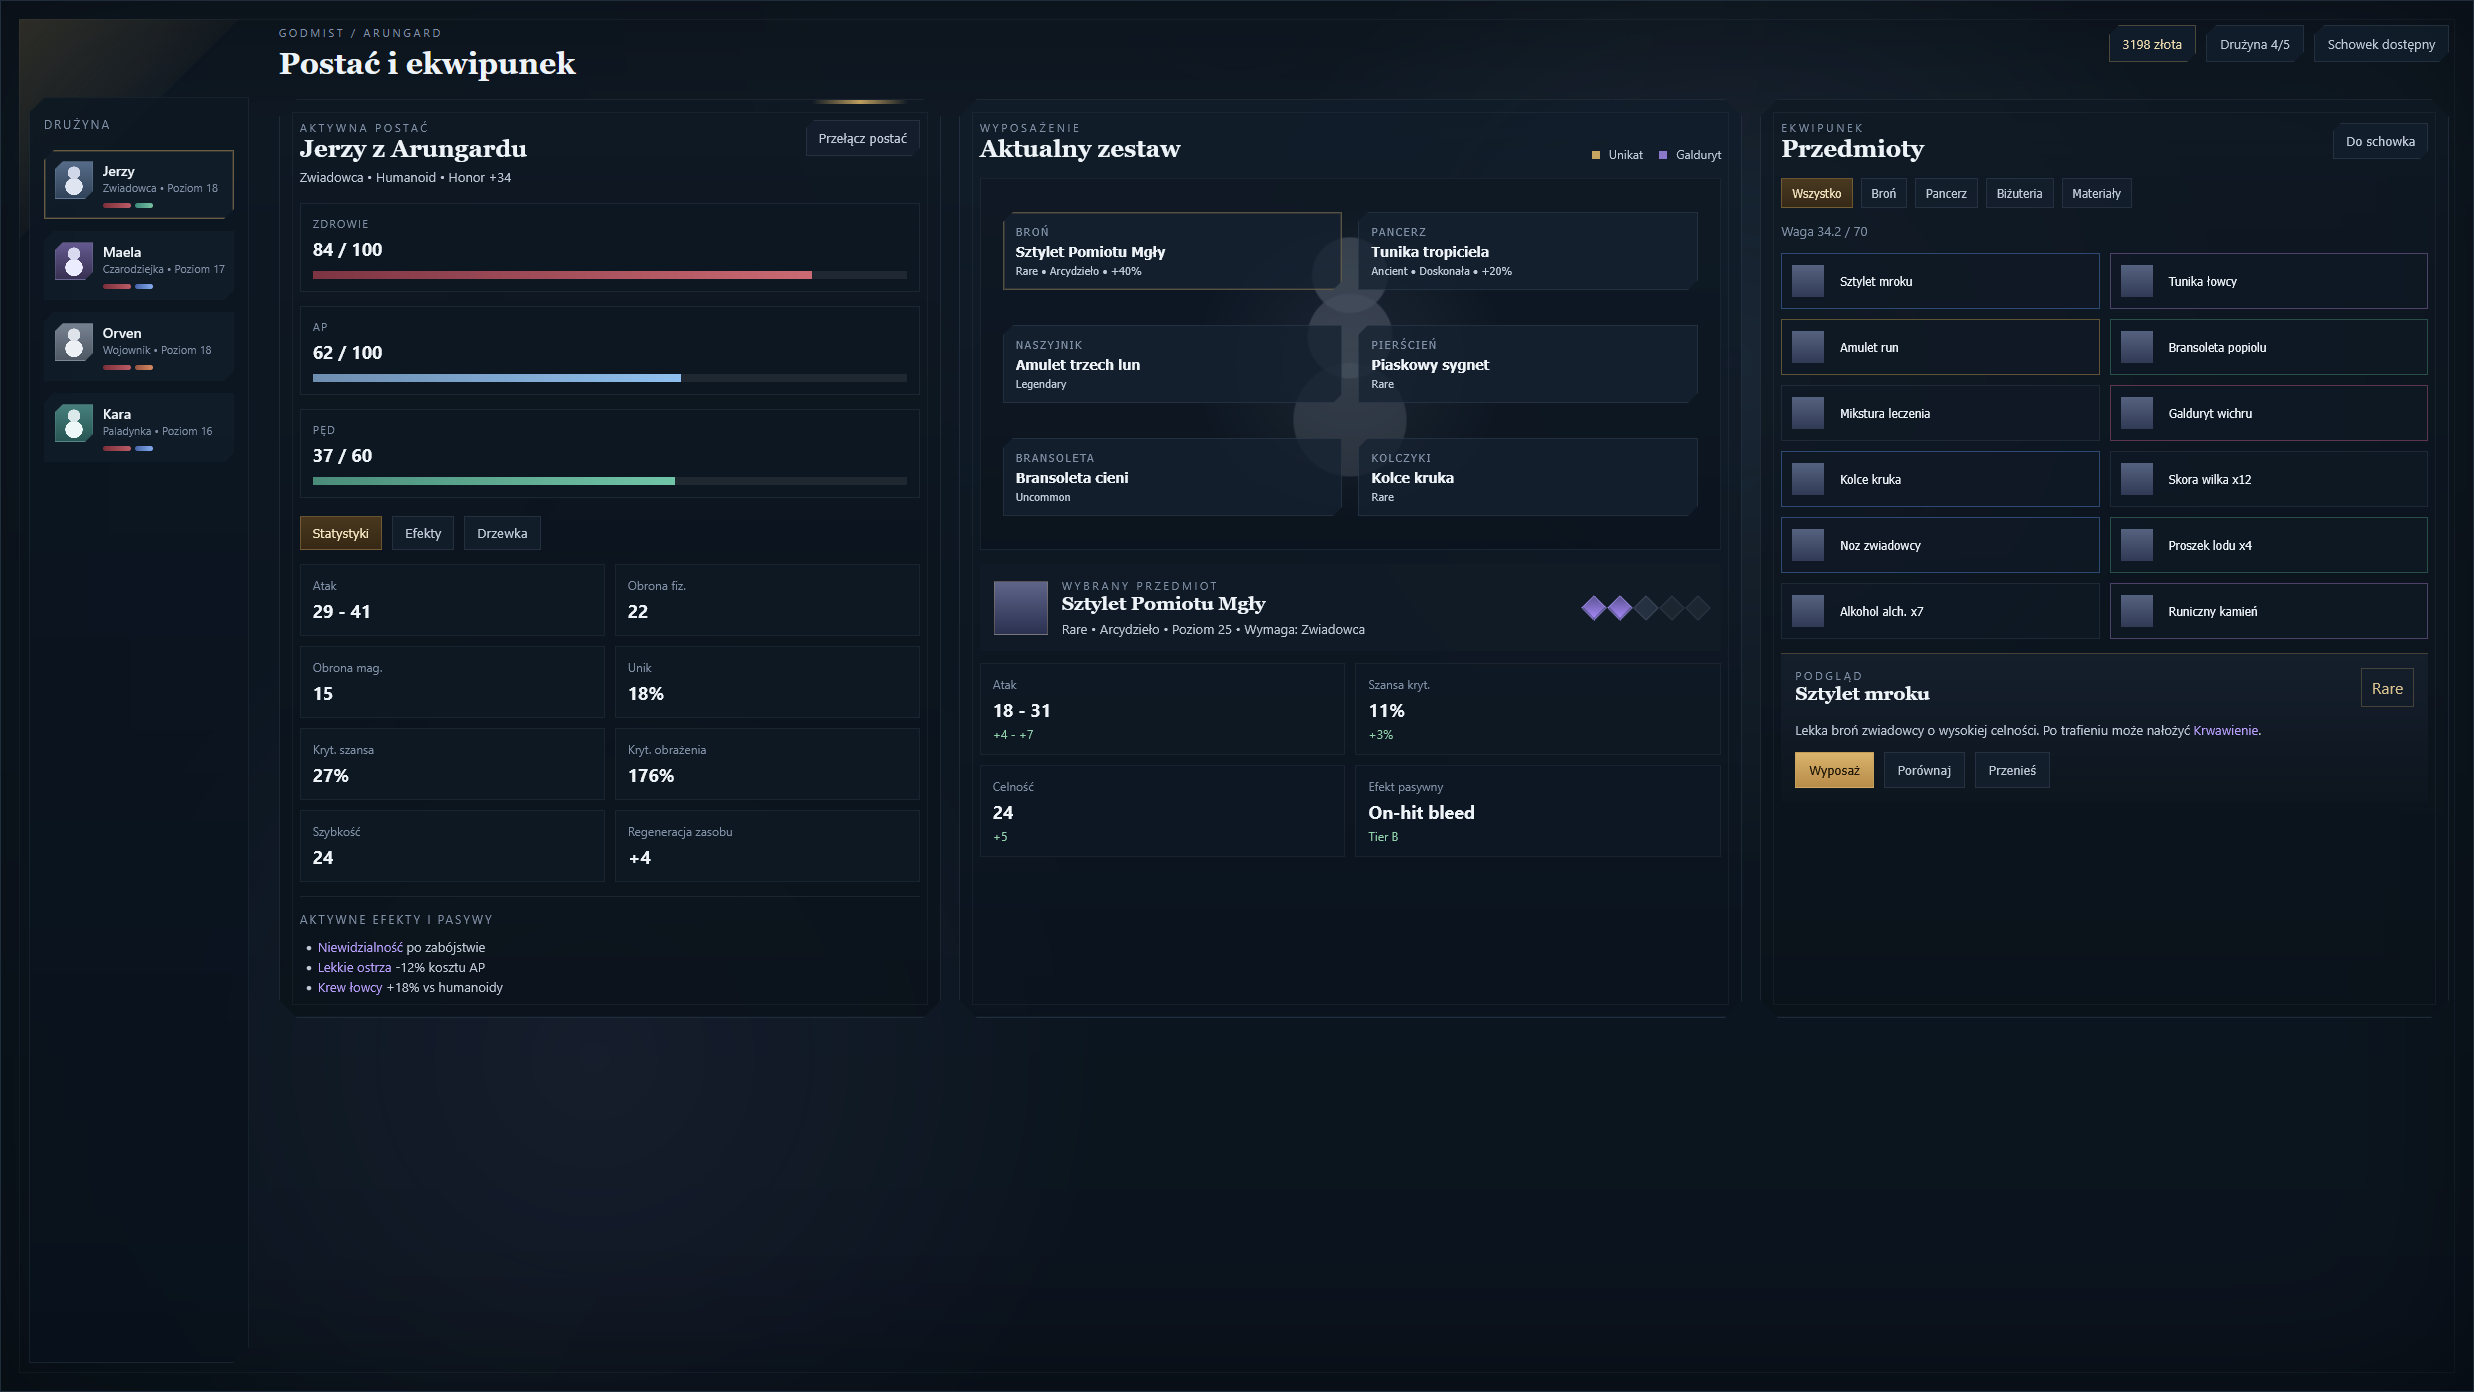
\includegraphics[width=\textwidth]{figures/gui/ui-character-equipment.png}
    \caption{Widok postaci i ekwipunku}
    \wsizsource{Opracowanie własne}
\end{figure}

Okno postaci i ekwipunku umożliwia przegląd statystyk, aktualnie założonych przedmiotów oraz zawartości ekwipunku. Centralnym elementem kompozycji jest sekcja wyposażenia postaci, natomiast informacje pomocnicze rozmieszczono po bokach w celu zachowania czytelności.

\begin{figure}[H]
    \centering
    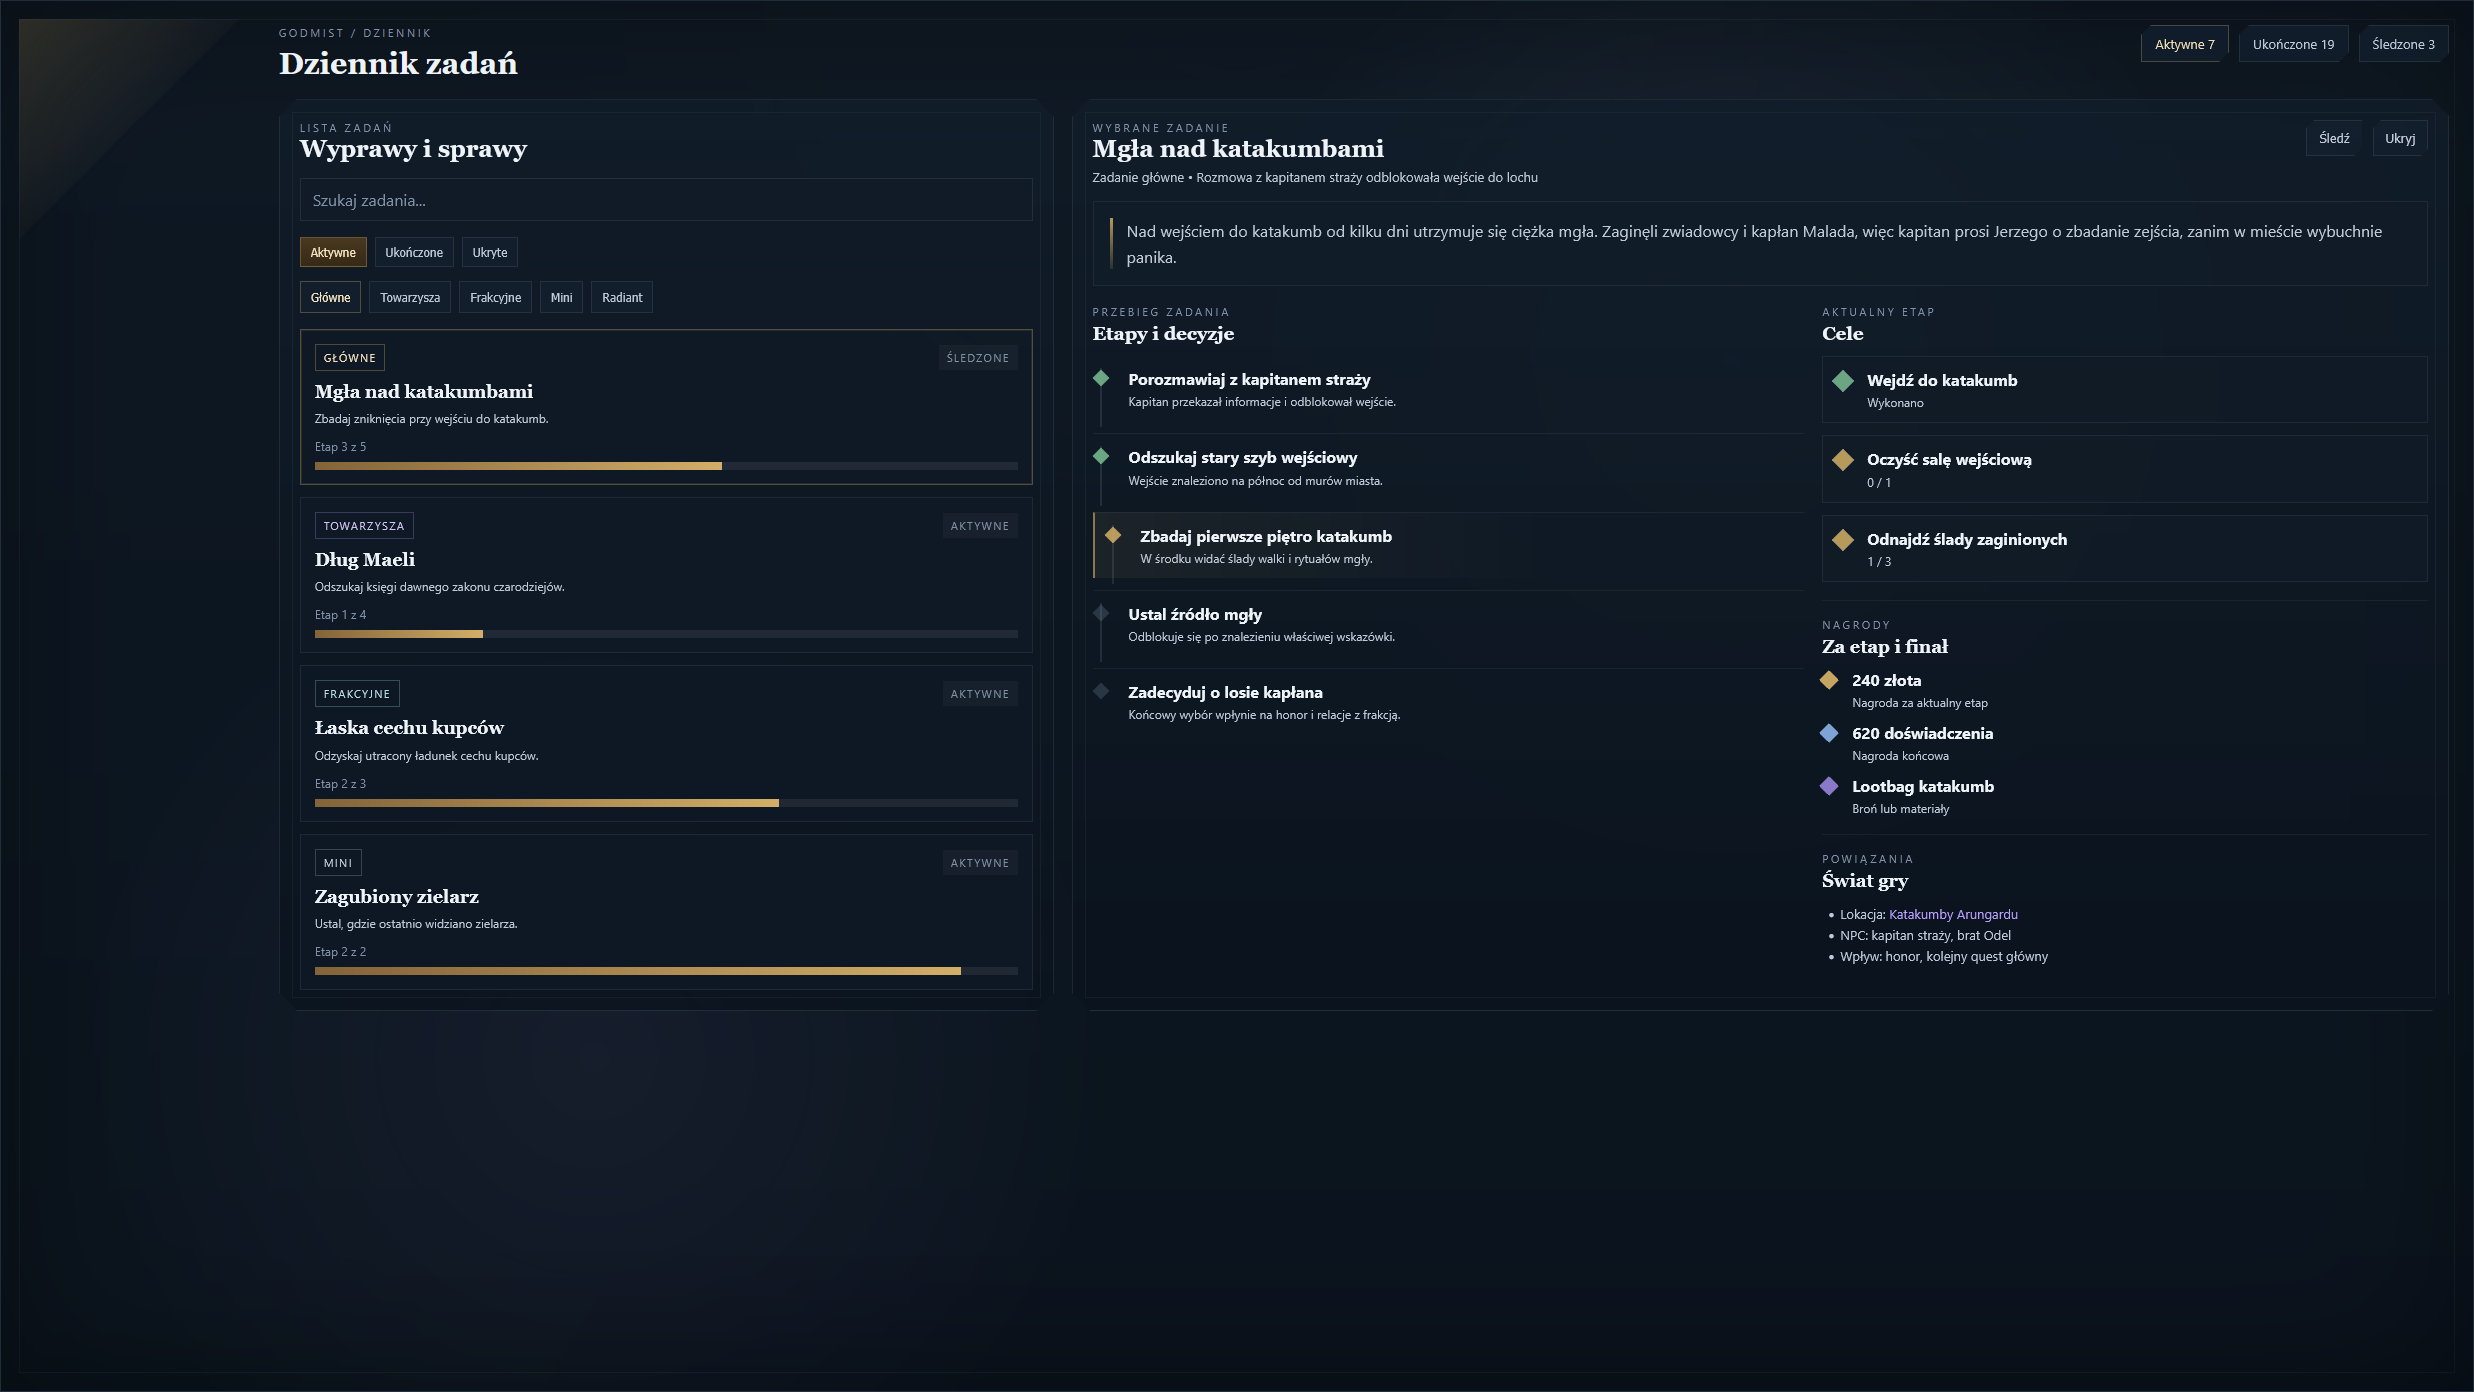
\includegraphics[width=\textwidth]{figures/gui/ui-quest-journal.png}
    \caption{Widok dziennika zadań}
    \wsizsource{Opracowanie własne}
\end{figure}

Dziennik zadań grupuje informacje o aktywnych i ukończonych misjach, ich etapach, nagrodach oraz powiązaniach ze światem gry. Układ kolumnowy pozwala oddzielić listę zadań od szczegółów aktualnie wybranego wpisu.

\begin{figure}[H]
    \centering
    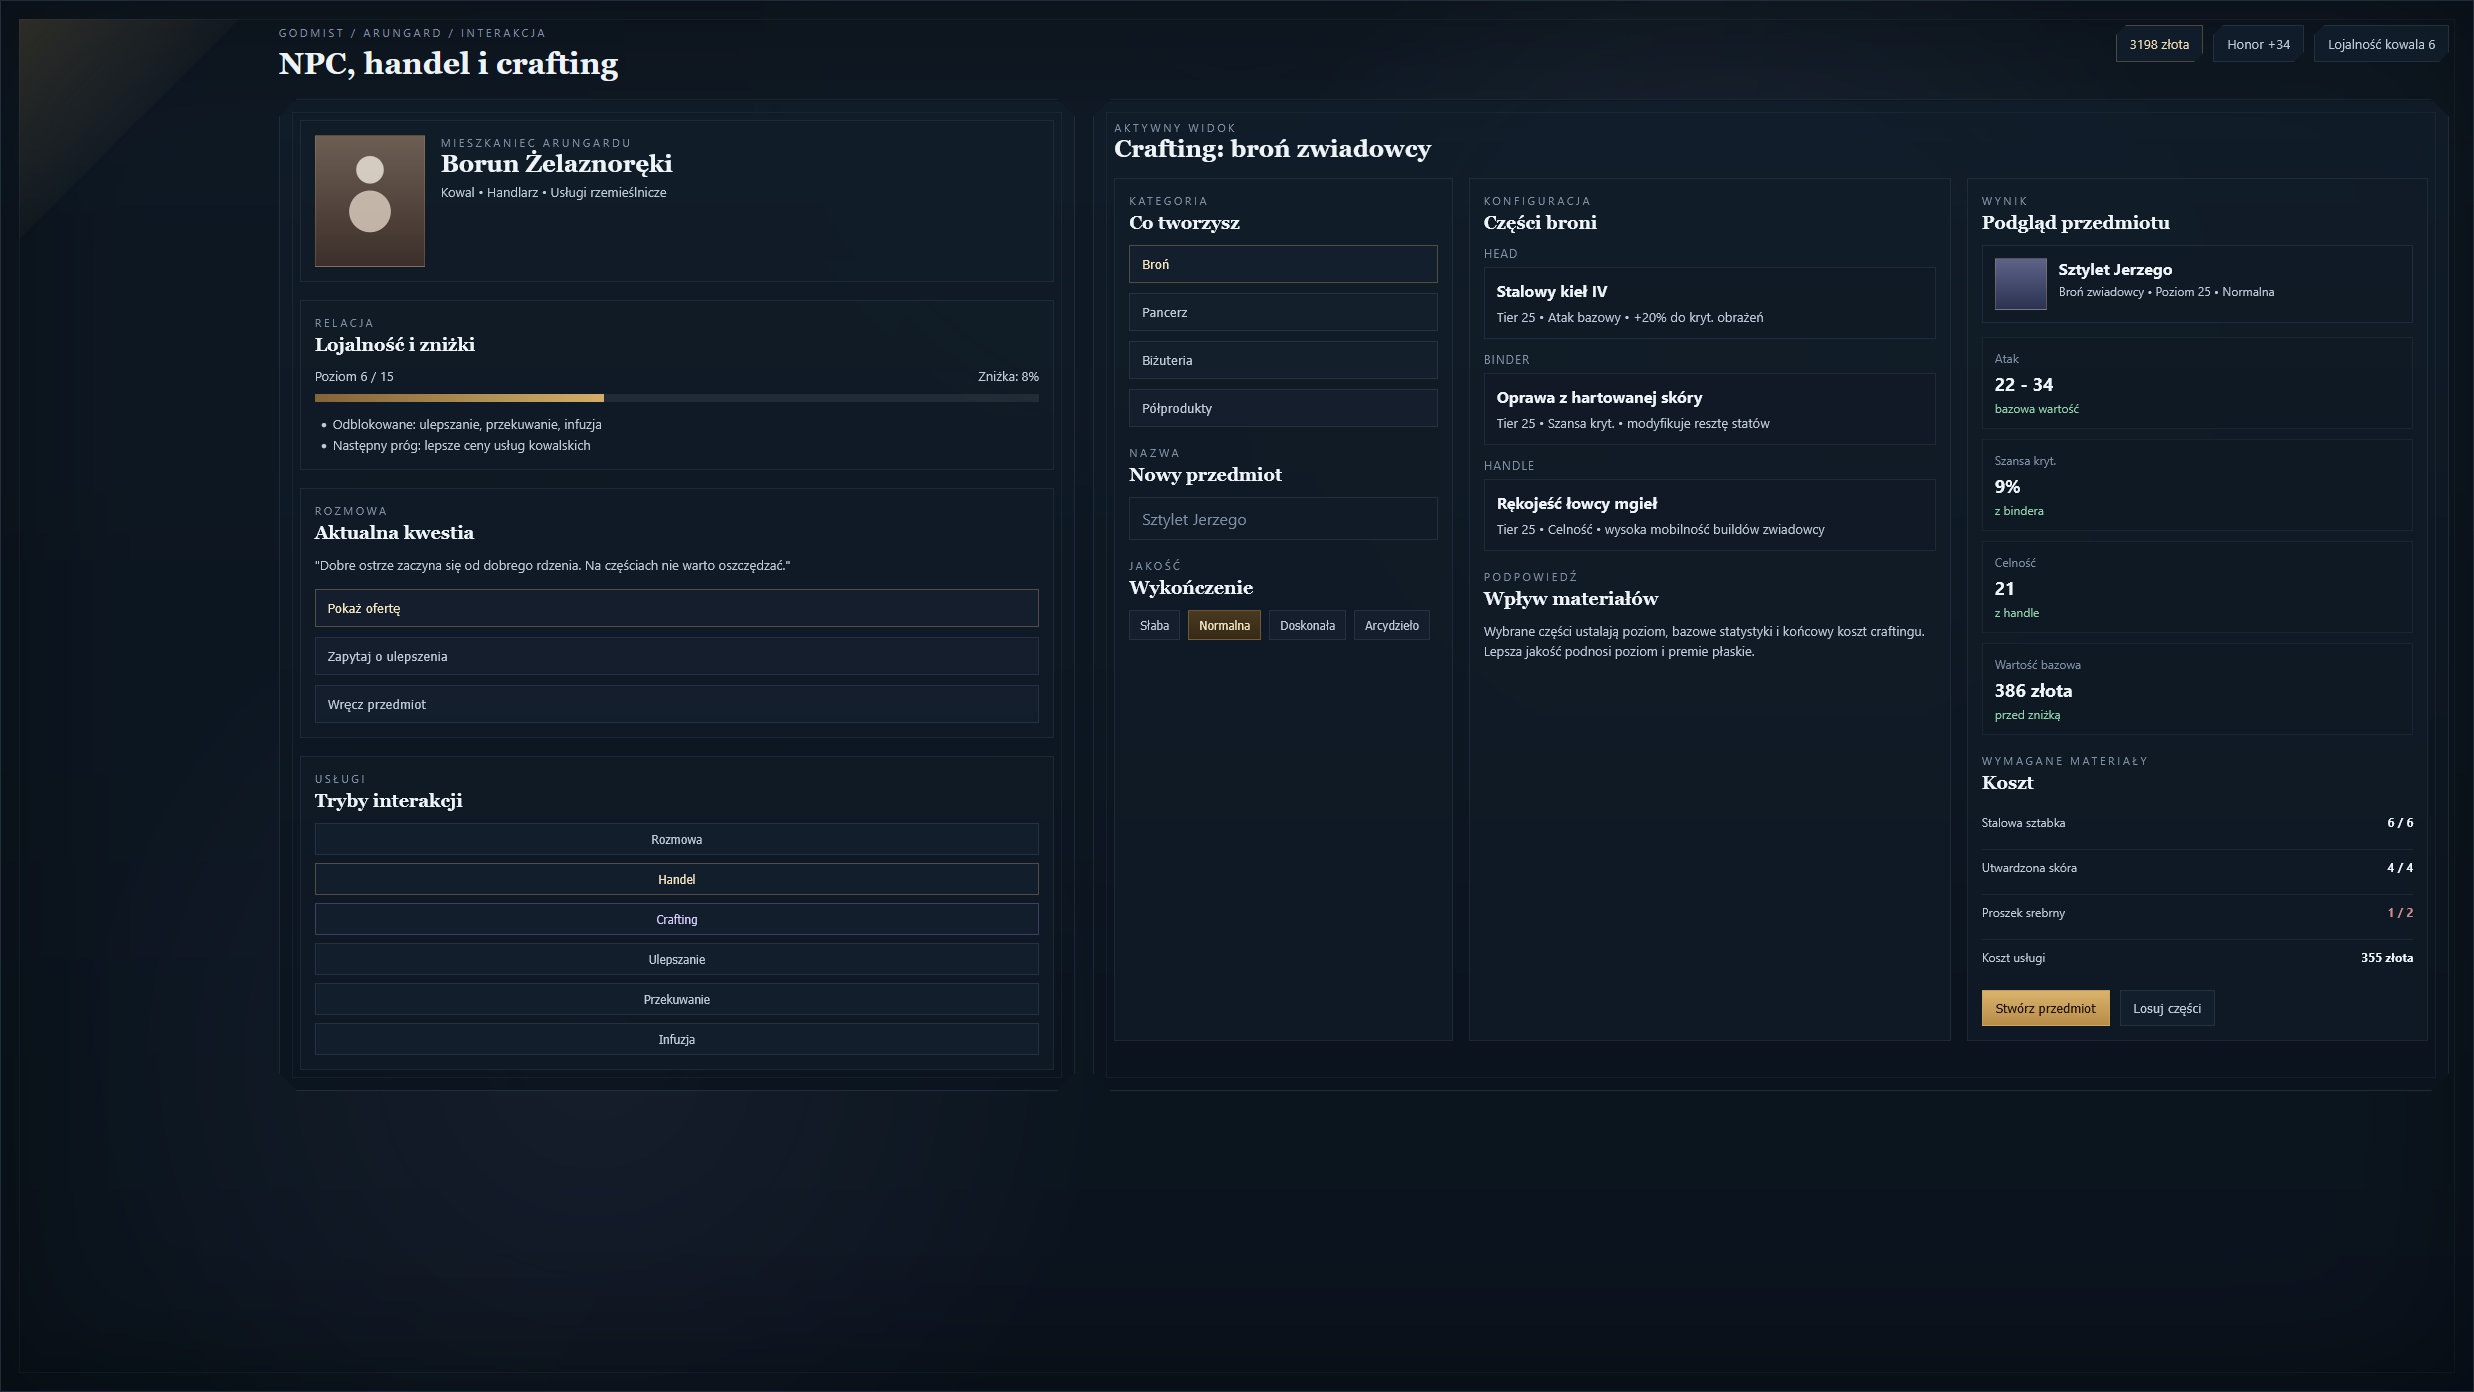
\includegraphics[width=\textwidth]{figures/gui/ui-npc-dialog.png}
    \caption{Widok interakcji z NPC}
    \wsizsource{Opracowanie własne}
\end{figure}

Okno interakcji z NPC stanowi wspólną bazę dla rozmowy, handlu oraz craftingu. Takie rozwiązanie upraszcza obsługę systemu i pozwala zachować spójność wizualną między różnymi usługami oferowanymi przez postacie niezależne.

\section{Propozycja testów}
\label{sec:propozycja-testow}

Ze względu na złożoność systemu \emph{Godmist} proces weryfikacji poprawności działania powinien obejmować kilka poziomów testowania. Oprócz sprawdzenia podstawowych funkcji dostępnych dla gracza konieczne jest również potwierdzenie poprawnej współpracy pomiędzy modułami systemu, prawidłowego działania zapisu i odczytu stanu gry oraz akceptowalnej wydajności rozwiązania. W niniejszej sekcji przedstawiono przykładowe scenariusze testowe, które mogą zostać wykorzystane podczas dalszej realizacji projektu.

Przedstawione przypadki testowe mają charakter projektowy. Oznacza to, że nie są jeszcze raportem z wykonanych testów, lecz propozycją zestawu sprawdzeń, które pozwolą zweryfikować zgodność implementacji z założeniami systemu. Dla czytelności testy podzielono na testy funkcjonalne, integracyjne, testy zapisu i odczytu oraz testy wydajnościowe i niezawodnościowe.

\subsection{Testy funkcjonalne}
\label{subsec:testy-funkcjonalne}

Testy funkcjonalne mają na celu sprawdzenie, czy system poprawnie realizuje najważniejsze funkcje widoczne z perspektywy użytkownika końcowego. Obejmują one między innymi rozpoczęcie gry, eksplorację lokacji, prowadzenie walki, rozwój postaci, korzystanie z ekwipunku oraz obsługę handlu i craftingu.

\begin{table}[H]
\centering
\caption{Przykładowe testy funkcjonalne systemu}
\label{tab:testy-funkcjonalne}
\begin{threeparttable}
\begin{tabularx}{\linewidth}{|p{1.6cm}|p{3.2cm}|X|X|X|}
\hline
\textbf{ID} & \textbf{Nazwa testu} & \textbf{Warunki początkowe} & \textbf{Kroki testowe} & \textbf{Oczekiwany rezultat} \\
\hline
TF-01 & Rozpoczęcie nowej gry & Aplikacja została uruchomiona, użytkownik znajduje się w menu głównym. & Wybrać opcję rozpoczęcia nowej gry. & System tworzy nową kampanię i przenosi gracza do początkowego stanu rozgrywki. \\
\hline
TF-02 & Eksploracja miasta & Gra została rozpoczęta, gracz znajduje się w mieście. & Poruszyć postać po mieście i wejść w interakcję z wybranym NPC. & Postać porusza się poprawnie, a interakcja z NPC otwiera odpowiedni panel lub dialog. \\
\hline
TF-03 & Rozpoczęcie walki w lochu & Gracz znajduje się w lochu i zbliża się do grupy przeciwników. & Wejść w zasięg przeciwnika inicjujący walkę. & System przełącza stan gry do trybu walki i inicjuje sesję combatową. \\
\hline
TF-04 & Użycie umiejętności w walce & Trwa walka, aktywna postać posiada wystarczające zasoby i punkty akcji. & Wybrać umiejętność i wskazać poprawny cel. & Umiejętność zostaje wykonana, a stan zasobów, punktów akcji i celu zostaje odpowiednio zaktualizowany. \\
\hline
TF-05 & Handel z NPC & Gracz znajduje się w mieście i posiada przedmiot oraz odpowiednią ilość złota. & Otworzyć sklep NPC, kupić oraz sprzedać wybrany przedmiot. & System poprawnie aktualizuje złoto, inventory gracza oraz stan sklepu i listy buyback. \\
\hline
TF-06 & Crafting przedmiotu & Gracz znajduje się przy odpowiednim NPC i posiada wymagane składniki. & Wybrać recepturę lub konfigurację przedmiotu i potwierdzić crafting. & System tworzy nowy przedmiot zgodnie z wybranymi parametrami i zużywa odpowiednie składniki. \\
\hline
TF-07 & Rozwój postaci & Postać posiada dostępne punkty rozwoju. & Otworzyć drzewko umiejętności i zainwestować punkt w wybrany node. & System zwiększa inwestycję w node, aktualizuje liczbę punktów i odblokowuje odpowiednie efekty. \\
\hline
\end{tabularx}
\wsizsource{Opracowanie własne}
\end{threeparttable}
\end{table}

\subsection{Testy integracyjne}
\label{subsec:testy-integracyjne}

Testy integracyjne służą do sprawdzenia poprawnej współpracy pomiędzy różnymi modułami systemu. W przypadku gry \emph{Godmist} ma to szczególne znaczenie, ponieważ wiele mechanik korzysta z tych samych danych runtime i oddziałuje na stan świata, postaci oraz przedmiotów.

\begin{table}[H]
\centering
\caption{Przykładowe testy integracyjne systemu}
\label{tab:testy-integracyjne}
\begin{threeparttable}
\begin{tabularx}{\linewidth}{|p{1.6cm}|p{3.2cm}|X|X|X|}
\hline
\textbf{ID} & \textbf{Nazwa testu} & \textbf{Warunki początkowe} & \textbf{Kroki testowe} & \textbf{Oczekiwany rezultat} \\
\hline
TI-01 & Walka i efekty statusu & Trwa walka, aktywna postać posiada umiejętność nakładającą status. & Użyć umiejętności nakładającej efekt statusu na przeciwnika. & System poprawnie nakłada status, zapisuje go w stanie postaci i uwzględnia jego działanie w kolejnych turach. \\
\hline
TI-02 & Ekwipunek i statystyki postaci & Postać posiada przedmiot zwiększający statystyki. & Założyć przedmiot na postać, a następnie go zdjąć. & Statystyki postaci zmieniają się po założeniu przedmiotu i wracają do poprzednich wartości po jego zdjęciu. \\
\hline
TI-03 & Quest i stan świata & Aktywna jest misja wymagająca interakcji z obiektem lub NPC. & Wykonać czynność wymaganą przez quest. & System aktualizuje postęp questa oraz odpowiednie flagi świata lub questa. \\
\hline
TI-04 & Loch i system walki & Gracz eksploruje loch zawierający encounter. & Wejść do pomieszczenia z przeciwnikami i ukończyć walkę. & System aktualizuje stan encountera w lochu i oznacza go jako ukończony. \\
\hline
TI-05 & Crafting i inventory & Gracz posiada wymagane materiały do craftingu. & Wytworzyć przedmiot u odpowiedniego NPC. & Materiały zostają zużyte, a nowy przedmiot trafia do odpowiedniego inventory. \\
\hline
\end{tabularx}
\wsizsource{Opracowanie własne}
\end{threeparttable}
\end{table}

\subsection{Testy zapisu i odczytu}
\label{subsec:testy-zapisu-i-odczytu}

Ze względu na przyjęty model trwałości danych oparty na plikach JSON, testy zapisu i odczytu należą do najważniejszych w całym projekcie. Ich celem jest weryfikacja, czy stan gry po zapisaniu i ponownym wczytaniu pozostaje zgodny ze stanem sprzed zakończenia sesji.

\begin{table}[H]
\centering
\caption{Przykładowe testy zapisu i odczytu}
\label{tab:testy-zapis-odczyt}
\begin{threeparttable}
\begin{tabularx}{\linewidth}{|p{1.6cm}|p{3.2cm}|X|X|X|}
\hline
\textbf{ID} & \textbf{Nazwa testu} & \textbf{Warunki początkowe} & \textbf{Kroki testowe} & \textbf{Oczekiwany rezultat} \\
\hline
TZ-01 & Zapis i wczytanie postaci & Postać posiada określony poziom, statystyki, ekwipunek i aktywne efekty. & Zapisać grę, zamknąć aplikację, a następnie wczytać zapis. & Po wczytaniu system odtwarza stan postaci zgodny ze stanem sprzed zapisu. \\
\hline
TZ-02 & Zapis i wczytanie lochu & Gracz znajduje się w lochu, odwiedził część pomieszczeń i ukończył wybrane encountery. & Zapisać grę i następnie wczytać zapis. & Stan lochu, w tym odwiedzone pomieszczenia i ukończone spotkania, zostaje odtworzony poprawnie. \\
\hline
TZ-03 & Zapis i wczytanie questów & Gracz posiada aktywne questy z częściowym postępem. & Zapisać grę i ponownie ją wczytać. & System poprawnie odtwarza status questów, cele oraz postęp wykonania. \\
\hline
TZ-04 & Zapis stanu NPC i handlu & NPC posiada określony poziom lojalności oraz stan sklepu i buybacku. & Zapisać grę po dokonaniu transakcji, a następnie ją wczytać. & Lojalność NPC, oferta sklepu i buyback pozostają zgodne z zapisanym stanem. \\
\hline
TZ-05 & Zapis schowka & W schowku znajdują się różne przedmioty. & Odłożyć przedmioty do schowka, zapisać grę i ponownie ją wczytać. & Schowek po wczytaniu zawiera ten sam zestaw przedmiotów. \\
\hline
\end{tabularx}
\wsizsource{Opracowanie własne}
\end{threeparttable}
\end{table}

\subsection{Testy wydajnościowe i niezawodnościowe}
\label{subsec:testy-wydajnosciowe}

Testy wydajnościowe i niezawodnościowe mają na celu ocenę stabilności systemu oraz sprawdzenie, czy podstawowe operacje nie powodują zauważalnych opóźnień lub błędów przy większej złożoności stanu gry. W przypadku projektu \emph{Godmist} istotne jest zwłaszcza zachowanie systemu przy rozbudowanym ekwipunku, wielu aktywnych efektach oraz przy obsłudze proceduralnie generowanych lochów.

\begin{table}[H]
\centering
\caption{Przykładowe testy wydajnościowe i niezawodnościowe}
\label{tab:testy-wydajnosciowe}
\begin{threeparttable}
\begin{tabularx}{\linewidth}{|p{1.6cm}|p{3.2cm}|X|X|X|}
\hline
\textbf{ID} & \textbf{Nazwa testu} & \textbf{Warunki początkowe} & \textbf{Kroki testowe} & \textbf{Oczekiwany rezultat} \\
\hline
TW-01 & Ładowanie lochu proceduralnego & System jest gotowy do wejścia do lochu. & Wygenerować i załadować loch proceduralny. & Loch zostaje wygenerowany i załadowany bez błędów, a czas oczekiwania pozostaje akceptowalny dla użytkownika. \\
\hline
TW-02 & Zapis dużego stanu gry & Gra zawiera rozwiniętą drużynę, dużą liczbę przedmiotów i aktywnych questów. & Wykonać zapis gry. & System zapisuje stan bez błędów i bez zauważalnego zawieszenia aplikacji. \\
\hline
TW-03 & Wczytanie dużego stanu gry & Istnieje zapis obejmujący rozbudowany stan świata i postaci. & Wczytać zapis gry. & System poprawnie odtwarza stan gry bez utraty danych i bez krytycznych opóźnień. \\
\hline
TW-04 & Stabilność długiej sesji gry & Użytkownik wykonuje wiele walk, interakcji i zapisów podczas jednej sesji. & Przeprowadzić dłuższą rozgrywkę obejmującą wiele przejść między modułami. & System zachowuje stabilność i nie wykazuje krytycznych błędów ani utraty spójności danych. \\
\hline
\end{tabularx}
\wsizsource{Opracowanie własne}
\end{threeparttable}
\end{table}

Przedstawiony zestaw testów nie wyczerpuje wszystkich możliwych scenariuszy weryfikacji systemu, ale stanowi reprezentatywną podstawę do dalszego planowania procesu testowania. Uwzględnia on zarówno działania wykonywane bezpośrednio przez użytkownika, jak i poprawność współpracy modułów, trwałość danych oraz stabilność techniczną systemu.

\section{Podsumowanie rozdziału}
\label{sec:podsumowanie-rozdzialu-3}

W niniejszym rozdziale przedstawiono założenia dotyczące interfejsu użytkownika projektowanego systemu oraz zaproponowano przykładowe scenariusze testowe, które mogą zostać wykorzystane podczas dalszej realizacji projektu. Omówiono najważniejsze widoki GUI związane z menu głównym, miastem, eksploracją lochu, walką oraz zarządzaniem ekwipunkiem i rozwojem postaci. Pozwoliło to określić, w jaki sposób użytkownik będzie komunikował się z systemem w różnych kontekstach rozgrywki.

Dodatkowo zaprezentowano propozycję testów funkcjonalnych, integracyjnych, testów zapisu i odczytu oraz testów wydajnościowych i niezawodnościowych. Dzięki temu projekt został uzupełniony o perspektywę weryfikacji poprawności działania poszczególnych modułów. Przedstawione elementy stanowią praktyczne dopełnienie wcześniejszych rozdziałów poświęconych analizie, wymaganiom oraz modelowi systemu.
\chapter{Podsumowanie}
\label{cha:podsumowanie}

W niniejszej pracy przedstawiono projekt systemu gry komputerowej \emph{Godmist} z perspektywy inżynierii oprogramowania. Opracowanie objęło analizę problemu, przegląd istniejących rozwiązań, określenie wymagań, modelowanie systemu, opis struktury danych, architektury rozwiązania, założeń interfejsu użytkownika oraz propozycji testów. Dzięki temu możliwe było przedstawienie projektu nie tylko jako koncepcji gry, ale również jako spójnego systemu informatycznego.

\section{Ocena realizacji założeń}
\label{sec:ocena-realizacji-zalozen}

Założony cel pracy został osiągnięty w zakresie przygotowania dokumentacji projektowej systemu. Opracowano model rozwiązania obejmujący najważniejsze mechaniki gry, takie jak eksploracja lochów, walka turowa, rozwój postaci, system ekwipunku, crafting, obsługa NPC, questy oraz trwałość stanu gry. Przygotowane modele pozwalają uporządkować zależności pomiędzy poszczególnymi elementami systemu i stanowią podstawę do dalszych prac implementacyjnych.

Istotnym rezultatem pracy jest również rozdzielenie projektu na warstwy odpowiedzialności, obejmujące definicje danych, stan runtime, serwisy systemowe, warstwę prezentacji oraz trwałość danych. Takie podejście sprzyja modularności rozwiązania i zwiększa jego podatność na dalszą rozbudowę.

\section{Wnioski końcowe}
\label{sec:wnioski-koncowe}

Przeprowadzona analiza pokazała, że projekt gry \emph{Godmist} wymaga integracji wielu współdziałających podsystemów, które muszą pozostawać ze sobą w zgodzie zarówno na poziomie logiki rozgrywki, jak i modelu danych. Z punktu widzenia inżynierii oprogramowania najważniejsze okazało się odpowiednie rozdzielenie definicji danych od zmiennego stanu gry oraz zaprojektowanie spójnej struktury pośredniczącej pomiędzy eksploracją, walką, przedmiotami, misjami i zapisem gry.

Dokumentacja przygotowana w ramach pracy porządkuje te zależności i tworzy podstawę do dalszej realizacji projektu. Można zatem uznać, że \emph{Godmist} został poprawnie opisany jako projekt systemu informatycznego o złożonej strukturze i wielu współzależnych modułach.

\section{Możliwe kierunki dalszego rozwoju}
\label{sec:kierunki-dalszego-rozwoju}

Projekt może być w przyszłości rozwijany zarówno od strony technicznej, jak i projektowej. Do najważniejszych kierunków dalszych prac należą:
\begin{itemize}
    \item pełna implementacja systemu w środowisku Unity,
    \item rozbudowa dialogów i warstwy fabularnej,
    \item rozwinięcie systemu lochów, przeciwników i zagadek,
    \item dalsze dopracowanie interfejsu użytkownika,
    \item rozszerzenie zestawu testów o testy wykonywane na działającej implementacji,
    \item balansowanie mechanik związanych z walką, rozwojem postaci i przedmiotami.
\end{itemize}

Przedstawiona dokumentacja może stanowić punkt wyjścia do dalszej realizacji projektu oraz kolejnych iteracji rozwojowych systemu.

%------------------------------------------------------------------------------
% Spisy (rysunki / tabele / listingi)
%------------------------------------------------------------------------------
\cleardoublepage
\addcontentsline{toc}{chapter}{Spis rysunków}
\listoffigures

\cleardoublepage
\addcontentsline{toc}{chapter}{Spis tabel}
\listoftables

\cleardoublepage
\addcontentsline{toc}{chapter}{Spis listingów}
\lstlistoflistings

%------------------------------------------------------------------------------
% Bibliografia
%------------------------------------------------------------------------------

\cleardoublepage
\selectlanguage{polish}
\begingroup
  \renewcommand{\emph}[1]{\textit{#1}}
  \addcontentsline{toc}{chapter}{Bibliografia}
  \nocite{*}
  \bibliographystyle{plain}
  \bibliography{bibliografia}
\endgroup
\renewcommand{\emph}[1]{\uline{#1}}


\end{document}
